\newpage

\section{Априорные распределения для задачи смеси экспертов}
В статье исследуется проблема построения смеси экспертов.
Смесь экспертов - это мультимодель, которая состоит из множества локальных моделей, которые называются экспертами и шлюзовой функции.
Смест экспертов использует шлюзовую функцию для взвешивания прогнозов каждого эксперта.
Весовые коэффициенты шлюзовую функции зависят от объекта, для которого производится прогноз.
Примерами мультимоделей являются бэггинг,  градиентный бустинг \cite{Tianqi2016} и случайный лес \cite{Ishwaran2012}.
В статье \cite{Yuksel2012} предполагается, что вклад каждого эксперта в ответ зависит от объекта из набора данных.

Основной проблемой построения мультимоделей является то, что ансамбль зависит от начальной инициализации параметров. Для улучшения устойчивости мультимодели предлагается использовать вероятностную постановку задачи для поиска оптимальных параметров шлюзовой функции и параметров локальной модели. В данной работе задается априорное распределения на параметры локальных моделей, также, для повышения, предлагается учесть зависимость априорных распределений для разных моделей.

\begin{figure}[h!t]\center
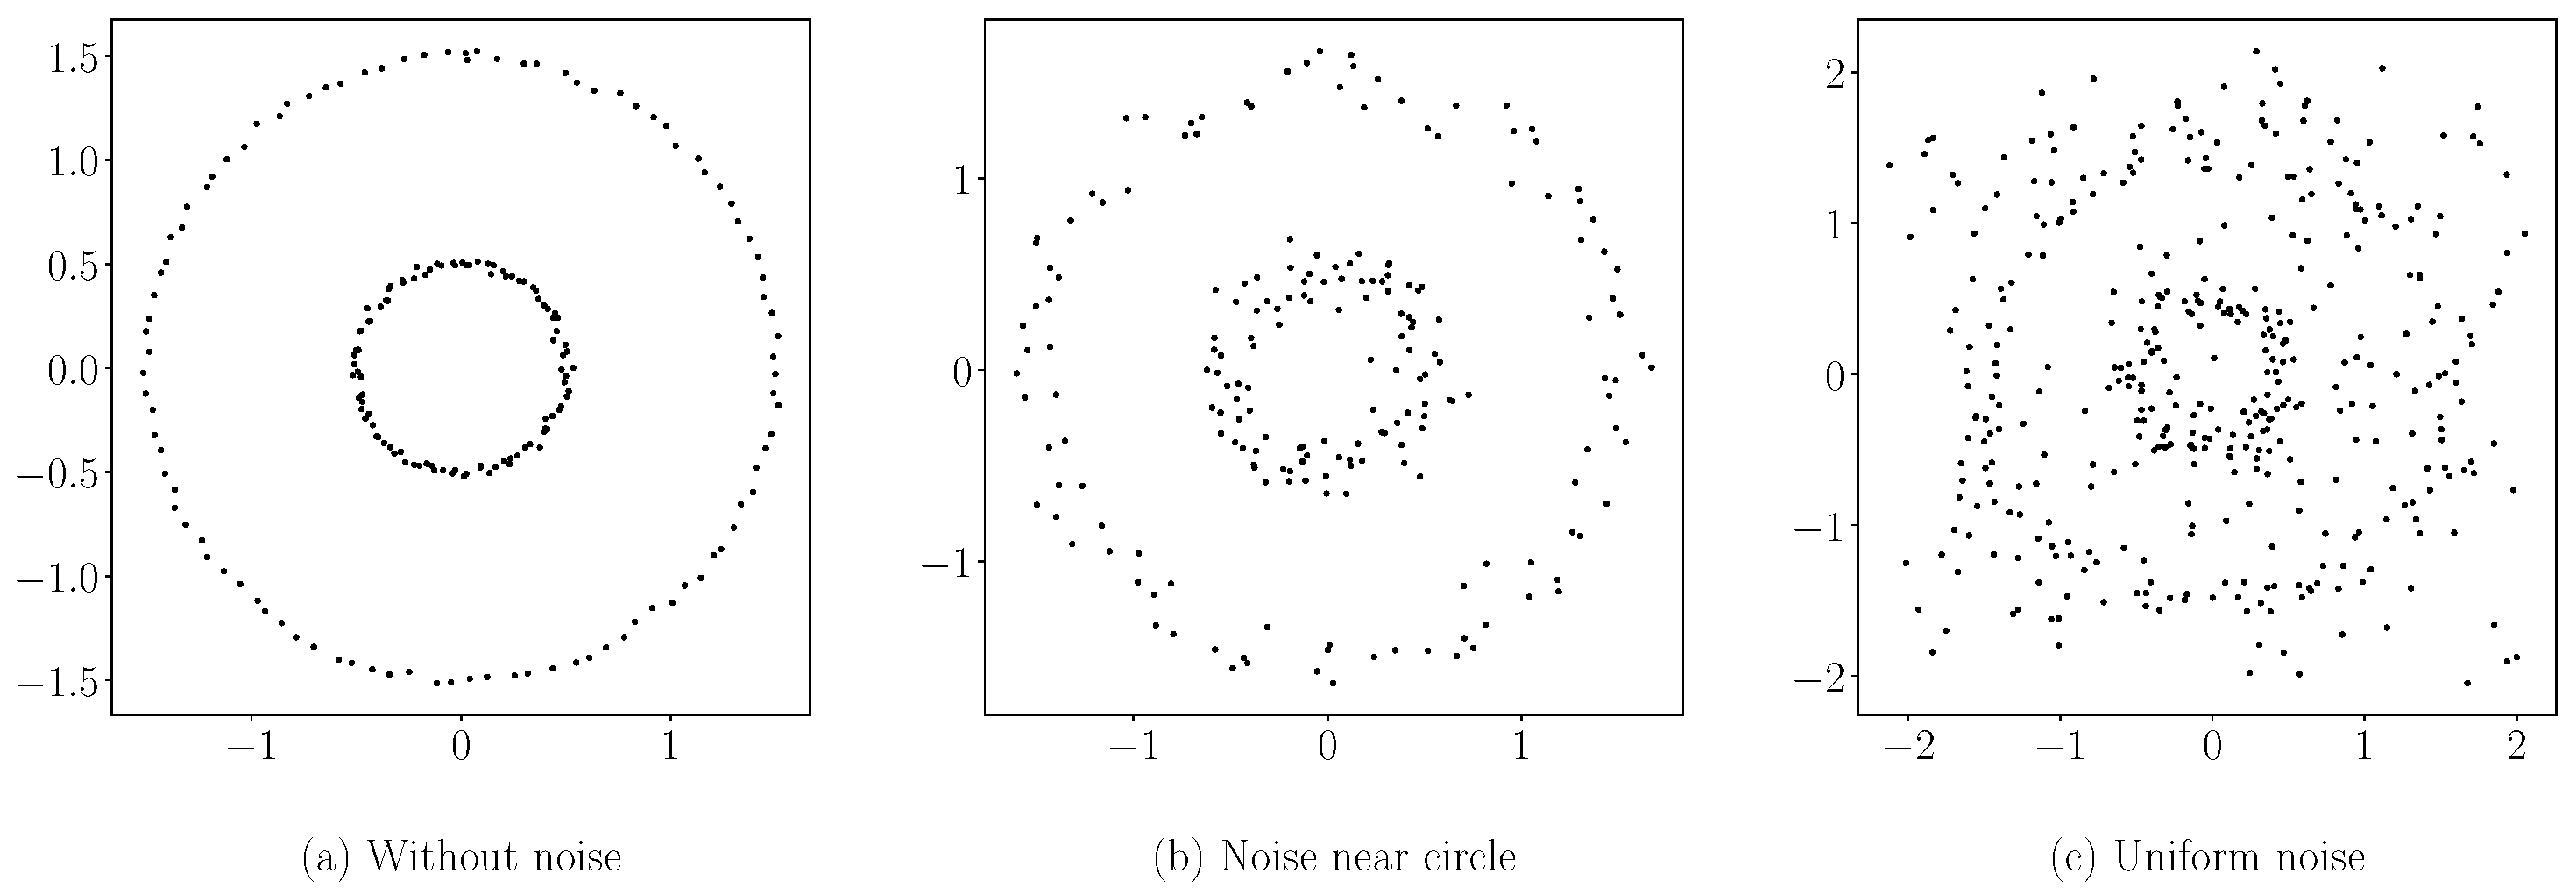
\includegraphics[width=1\textwidth]{results/priorexpert/statment}
\caption{Пример окружностей с разным уровнем шума: (a) окружности без шума; (b) окружности с зашумленным радиусом; (c) окружности с зашумленным радиусом, а также с равномерным шумом по всему изображению}
\label{example:1}
\end{figure}

В данной работе решается задача поиска окружностей на бинаризованном изображении. Предполагается, что радиусы окружностей различаются значимо, а также, что центры почти совпадают. Пример изображений показан на рис. \ref{example:1}. В данной работе в качестве экспертов рассматриваются линейные модели --- каждая модель аппроксимирует одну окружности. В качестве шлюзовой функции рассматривается двухслойная нейронная сеть.

Большое количество работ в области построения смеси экспертов посвящены выбору шлюзовой функции: используется softmax, процесс Дирихле \cite{Edward2002}, нейронная сеть \cite{Shazeer2017} с функцией softmax на последнем слое. Ряд работ посвящены выбору моделей в качестве отдельных экспертов. В работах \cite{Jordan1994, Jordan1991} в качестве модели эксперта рассматривается линейная модель. Работы \cite{Lima2007, Cao2003} рассматриваю модель SVM в качестве модели эксперта.
В работе \cite{Yuksel2012} представлен обзор методов и моделей в задачах смеси экспертов.

Смесь экспертов имеет множество приложений в прикладных задачах. Работы \cite{Yumlu2003, Cheung1995, Weigend2000} посвящены применению смеси экспертов в задачах прогнозирования временных рядов. 
В работе \cite{Ebrahimpour2009} предложен метод распознавания рукописных цифр. 
Метод распознания текстов при помощи смеси экспертов иследуется в работах \cite{Estabrooks2001}, распознание речи \cite{Mossavat2010, Peng1996, Tuerk2001}. 
В работе \cite{Sminchisescu2007} исследуется смесь экспертов для задачи распознавания трехмерных движений человека. 
В \cite{Bowyer2010} описаны работы по исследованию обнаружения радужки глаза на изображении. В работах \cite{Matveev2010, Matveev2014} в частности описаны методы выделения границ радужки и зрачка.

\subsection{Постановка задачи аппроксимации параметров окружности}
Задано бинарное изображение
\[
\label{eq:st:cr:1}
\begin{aligned}
\textbf{M} \in \{0,1\}^{m_1 \times m_2},
\end{aligned}
\]
где $1$ --- это черный пиксель, который принадлежит рассматриваемой фигуре на изображении, а $0$ --- белый пиксель, который является фоном изображения. 
Пример изображения показан на рис. \ref{example:1}.
Изображение $\textbf{M}$ отображается в множество координат \mbox{$\textbf{C}=\left\{x_i, y_i\right\}_{i=1}^{N}$}. Координата $(x_i, y_i)$ является координатой $i$-го черного пикселя на изображении $\textbf{M}$:
\[
\label{eq:st:cr:2}
\begin{aligned}
\textbf{C} \in  \mathbb{R}^{N \times 2},
\end{aligned}
\]
где $N$ --- число черных пикселей.

Обозначим точку $(x_0, y_0)$ центром окружности, а $r$ радиусом окружности.
Координаты $\left(x_i, y_i\right)\in\textbf{C}$ это геометрическое место точек, которое удовлетворяет системе уравнений:
\[
\label{eq:st:cr:3}
\begin{aligned}
\bigr(x_i - x_0\bigr)^{2}+\bigr(y_i-y_0\bigr)^2 = r^2 + \varepsilon_i, \qquad \forall i \in \{1, \cdots, N\},
\end{aligned}
\]
где $\varepsilon_i \in \mathcal{N}\bigr(0, \beta^{-1}\bigr)$ является невязкой $i$-го уравнения, которая является следствием шума на изображении.

Раскрыв скобки получаем:
\[
\label{eq:st:cr:4}
\begin{aligned}
\left(2x_0\right)\cdot x_i + \left(2y_0\right)\cdot y_i+\left(r^2-x_0^2-y_0^2\right)\cdot1 = x_{i}^2 + y_{i}^2 + \varepsilon_i.
\end{aligned}
\]
Выражение \eqref{eq:st:cr:4} переписывается в задачу линейной регрессии следующим образом:
\[
\label{eq:st:cr:5}
\begin{aligned}
\hat{\textbf{w}} = \arg\min_{\textbf{w}\in \mathbf{R}^{n}}||\textbf{X}\textbf{w} - \textbf{y}||,  \quad \textbf{X} = \left[\textbf{C}, \textbf{1}\right], \quad \textbf{y} = \left[x_1^2+y_1^2, x_2^2+y_2^2, \cdots, x_N^2+y_N^2\right]^{\mathsf{T}}.
\end{aligned}
\]
Используя вектор параметров $\hat{\textbf{w}} = \left[w_1, w_2, w_3\right]^{\mathsf{T}}$ получим параметры окружности $x_0, y_0, r$:
\[
\label{eq:st:cr:6}
\begin{aligned}
x_0 = \frac{w_1}{2}, \quad y_0 = \frac{w_2}{2}, \quad r = \sqrt[]{w_3+x_{0}^{2}+y_{0}^{2}}.
\end{aligned}
\]
Решение уравнения \eqref{eq:st:cr:5} находит параметры единственной окружности на изображении. В случае, когда на изображении несколько окружностей, предлагается использовать смесь экспертов, которая состоит из линейных модели --- экспертов. Каждый эксперт описывает одну окружность на изображении.

Обобщим подход аппроксимации одной окружности на изображении на случай, когда на изображении несколько окружностей. Пусть изображение состоит из $K$ окружностей, тогда множество черных пикселей $\textbf{C}$ представляется в виде:
\[
\label{eq:st:1}
\begin{aligned}
\textbf{C} = \sqcup_{k=1}^{K}\textbf{C}_{k}',
\end{aligned}
\]
где $\textbf{C}_{k}'$ множество точек принадлежащих $k$-й окружности. Множеству точек $\textbf{C}_{k}' \subset\textbf{C}$ соответсвует задача линейной регрессии для выборки $\textbf{X}_{k}' \subset \textbf{X}, \textbf{y}_{k}' \subset \textbf{y}$. Модель $\mathbf{g}_k$ аппроксимирующая выборку $\textbf{X}_{k}', \textbf{y}_{k}'$ является локальной моделью для выборки \textbf{X}, \textbf{y}.


\begin{definition}
\label{def:1}
Модель $\mathbf{g}$ называется локальной моделью для выборки $\textbf{U},$ если $\mathbf{g}$ аппроксимирует некоторое не пустое подмножество $\textbf{U}'\subset\textbf{U}$.
\end{definition}

\begin{definition}
\label{def:2}
Мультимодель $\mathbf{f}$ называется смесью экспертов, если:
\[
\label{eq:st:2}
\begin{aligned}
\mathbf{f} = \sum_{k=1}^{K}\pi_{k}\mathbf{g}_k\bigr(\mathbf{w}_k\bigr), \qquad \pi_{k}\bigr(\mathbf{x}, \mathbf{V}\bigr):\mathbb{R}^{n\times \left|\mathbf{V}\right|} \to [0, 1], \qquad \sum_{k=1}^{K}\pi_{k}\bigr(\mathbf{x}, \mathbf{V}\bigr) = 1,
\end{aligned}
\]
где $\mathbf{g}_k$ является $k$-й локальной моделью, $\pi_k$ --- шлюзовая функция, вектор $\mathbf{w}_k$ является параметрами $k$-й локальной моделью, а $\mathbf{V}$ --- параметры шлюзовой функции.
\end{definition}

В данной работе в качестве локальных моделей рассматриваются линейные модели. В качестве шлюзовой функции рассматривается двухслойный перцептрон:
\[
\label{eq:st:3}
\begin{aligned}
\mathbf{g}_k\bigr(\textbf{x}\bigr) = \textbf{w}_k^{\mathsf{T}}\textbf{x}, \quad
\bm{\pi}\bigr(\mathbf{x}, \mathbf{V}\bigr) = \text{softmax}\bigr(\mathbf{V}_{1}^{\mathsf{T}}\bm{\sigma}\bigr(\mathbf{V}_2^{\mathsf{T}}\mathbf{x}\bigr)\bigr),
\end{aligned}
\]
где $\mathbf{V} = \bigr\{\mathbf{V}_1, \mathbf{V}_2\bigr\}$ --- множество параметров шлюзовой функции.

В статье предлагается использовать вероятностный подход для описания смеси экспертов. Вводиться предположение, что $\textbf{y}$ является случайным вектором, который задается плотностью распределения $p\bigr(\textbf{y}|\textbf{X}\bigr)$. Предполагается, что плотность распределения $p\bigr(\textbf{y}|\textbf{X}, \textbf{f}\bigr)$ аппроксимирует истинную плотность распределения $p\bigr(\textbf{y}|\textbf{X}\bigr)$:
\[
\label{eq:st:new:1}
\begin{aligned}
p\bigr(\textbf{y}|\textbf{X}, \textbf{f}\bigr) = \prod_{i=1}^{N}\left(\sum_{k=1}^{K}\pi_kp_{k}\bigr(y_{i}|\textbf{g}_{k}\bigr(\mathbf{x}_{i}\bigr)\bigr)\right),
\end{aligned}
\]
где $\textbf{f}$ --- это смесь экспертов, а $\textbf{g}_k, \bm{\pi}$ определяются выражением \eqref{eq:st:3}.

Пусть $\textbf{w}_k$ является случайным вектором, который задается плотностью распределения $p^{k}\bigr(\mathbf{w}_k\bigr)$. Получим совместное распределения параметров локальных моделей и вектора ответов:
\[
\label{eq:st:4}
\begin{aligned}
p\bigr(\mathbf{y}, \mathbf{W}|\mathbf{X}, \mathbf{V}\bigr) = \prod_{k=1}^{K}p^{k}\bigr(\mathbf{w}_k\bigr)\prod_{i=1}^{N}\left(\sum_{k=1}^{K}\pi_{k}p_{k}\bigr(y_i|\mathbf{w}_k, \mathbf{x}_i\bigr)\right),
\end{aligned}
\]
где $\mathbf{W} = \bigr\{\mathbf{w}_1, \mathbf{w}_2, \cdots, \mathbf{w}_K\bigr\}.$
Оптимальные параметры находятся при помощи максимизации правдоподобия:
\[
\label{eq:st:5}
\begin{aligned}
\hat{\mathbf{V}}, \hat{ \mathbf{W}} = \arg\max_{\mathbf{V}, \mathbf{W}} p\bigr(\mathbf{y},  \mathbf{W}|\mathbf{X}, \mathbf{V}\bigr).
\end{aligned}
\]

\subsection{Вероятностная постановка задачи смеси экспертов}
Для построения смеси экспертов (\ref{eq:st:2},  \ref{eq:st:4}), введем следующие вероятностные предположения о данных \eqref{eq:st:cr:5}:

\begin{enumerate}
	\item[1)] правдоподобие $p_{k}\bigr(y_{i}|\mathbf{w}_{k}, \mathbf{x}_{i}\bigr) = \mathcal{N}\bigr(y_{i}|\mathbf{w}_{k}^{\mathsf{T}}\mathbf{x}_{i}, \beta^{-1}\bigr),$ где параметр $\beta$ является уровнем шума,
	\item[2)] априорное распределение параметров $p^{k}\bigr(\mathbf{w}_{k}\bigr) = \mathcal{N}\bigr(\mathbf{w}_{k}|\mathbf{w}^{0}_{k}, \mathbf{A}_{k}\bigr),$ где $\mathbf{w}^{0}_{k}$ --- вектор размерности $n\times1$, а  $\mathbf{A}_{k}$ --- ковариационная матрица размерности $n\times n$,
	\item[3)] регуляризация априорного распределения $p\bigr(\bm{\varepsilon}_{k,k'}|\bm{\Xi}\bigr) = \mathcal{N}\bigr(\bm{\varepsilon}_{k,k'}|\mathbf{0},  \bm{\Xi}\bigr),$ где $\bm{\Xi}$ --- ковариационная матрица, а $\bm{\varepsilon}_{k,k'} = \mathbf{w}_{k}^{0}-\mathbf{w}_{k'}^{0}.$
\end{enumerate}
Предположение 2) задает априорное предположения на вектора параметров локальных модели $\textbf{w}_k$. Априорное распределение  задает ограничения на локальную модель. Например, если $\textbf{w}_k^{0} = [0,0,1]$, то $k$-я локальная модель аппроксимирует окружность с параметрами $x_0=0, y_0=0, r=1$ с большей вероятностью.

Предположения 3) задает регулярицию априорных распределений. Данная регулярицая учитывает связь между априорными ограничениями разных локальных моделей. Например, если $\text{diag}\bigr(\bm{\Xi}\bigr)=[0.001, 0.001, 1]$, то  центры разных окружностей совпадают.

Используя предположения $1), 2), 3)$ и выражение \eqref{eq:st:4} получаем полное правдоподобие:
\[
\label{eq:em:1}
\begin{aligned}
p\bigr(\mathbf{y}, \mathbf{W}|\mathbf{X}, \mathbf{V}, \textbf{A}, \textbf{W}^{0}, \bm{\Xi}, \beta\bigr) = &\prod_{i=1}^{N}\left(\sum_{k=1}^{K}\pi_{k}\mathcal{N}\bigr(y_{i}|\mathbf{w}_{k}^{\mathsf{T}}\mathbf{x}_{i}, \beta^{-1}\bigr)\right)\cdot\\
&\cdot\prod_{k=1}^{K}\mathcal{N}\bigr(\mathbf{w}_{k}|\mathbf{w}^{0}_{k}, \mathbf{A}_{k}\bigr)\cdot\prod_{k,k'=1}^{K}\mathcal{N}\bigr(\bm{\varepsilon}_{k,k'}|\mathbf{0},  \bm{\Xi}\bigr),
\end{aligned}
\]

 где $\mathbf{A} = \left\{\mathbf{A}_1, \cdots, \mathbf{A}_K\right\}.$
 
Введем бинарную матрицу $\mathbf{Z}$. Элемент матрицы $z_{ik}$ равно $1$ тогда и только тогда, когда $i$-й объект аппроксимируется $k$-й локальной моделью.
Подставляя бинарную матрицу $\mathbf{Z}$ в выражении \eqref{eq:em:1}, а также взяв логарифм получаем:
\[
\label{eq:em:2}
\begin{aligned}
\log p\bigr(\mathbf{y}, \mathbf{Z}, \mathbf{W}&|\mathbf{X}, \mathbf{V}, \textbf{A}, \textbf{W}^{0},  \bm{\Xi}, \beta\bigr) =\\
&= \sum_{i=1}^{N}\sum_{k=1}^{K}z_{ik}\left[\log\pi_k\bigr(\textbf{x}_i, \textbf{V}\bigr) - \frac{\beta}{2}\left(y_{i} - \textbf{w}_{k}^{\mathsf{T}}\textbf{x}_{i}\right)^{2} + \frac{1}{2}\log\frac{\beta}{2\pi}\right] +\\
&+ \sum_{k=1}^{K}\left[-\frac{1}{2}\left(\textbf{w}_{k} - \textbf{w}_{k}^{0}\right)^{\mathsf{T}}\textbf{A}_{k}^{-1}\left(\textbf{w}_{k} - \textbf{w}_{k}^{0}\right) + \frac{1}{2}\log\det\textbf{A}^{-1}_{k} - \frac{n}{2}\log2\pi\right]+\\
&+ \sum_{k=1}^{K}\sum_{k'=1}^{K}\left[-\frac{1}{2}\left(\textbf{w}_{k}^{0}-\textbf{w}_{k'}^{0}\right)^{\mathsf{T}}\bm{\Xi}^{-1}\left(\textbf{w}_{k}^{0}-\textbf{w}_{k'}^{0}\right) +\frac{1}{2}\log\det \bm{\Xi} -\frac{n}{2}\log{2\pi}\right].
\end{aligned}
\]
Получаем новую задачу оптимизации обоснованности. Функция обоснованности получается при интегрировании выражения \eqref{eq:em:2} по параметрам $\textbf{W}, \textbf{Z}$:
\[
\label{eq:em:3}
\begin{aligned}
\mathbf{V}, \mathbf{W}^0, \textbf{A},  \beta = \arg\max_{\mathbf{V}, \mathbf{W}^0, \textbf{A}, \beta} \int_{\textbf{W}, \textbf{Z}}\log p\bigr(\mathbf{y}, \textbf{Z}, \textbf{W}|\mathbf{X}, \mathbf{V}, \textbf{A}, \textbf{W}^{0}, \bm{\Xi}, \beta\bigr)d\textbf{W}d\textbf{Z}.
\end{aligned}
\]
Рассмотрим вариационную плотность $q\bigr(\textbf{W}, \textbf{Z}\bigr)$ для параметров $\textbf{W}, \textbf{Z}$. Тогда функция обоснованности принимает следующий вид:
\[
\label{eq:em:new:1}
\begin{aligned}
\log p\bigr(\mathbf{y}|\mathbf{X}, \mathbf{V}, \textbf{A}, \textbf{W}^{0}, \bm{\Xi}, \beta\bigr) &= \int_{\textbf{W}, \textbf{Z}} q\bigr(\textbf{W}, \textbf{Z}\bigr) \log p\bigr(\mathbf{y}|\mathbf{X}, \mathbf{V}, \textbf{A}, \textbf{W}^{0}, \bm{\Xi}, \beta\bigr)d\textbf{W}d\textbf{Z} =\\
&= \int_{\textbf{W}, \textbf{Z}} q\bigr(\textbf{W}, \textbf{Z}\bigr)\log \frac{p\bigr(\mathbf{y}, \textbf{W}, \textbf{Z}|\mathbf{X}, \mathbf{V}, \textbf{A}, \textbf{W}^{0}, \bm{\Xi}, \beta\bigr)}{p\bigr(\textbf{W}, \textbf{Z}|\mathbf{y}, \mathbf{X}, \mathbf{V}, \textbf{A}, \textbf{W}^{0}, \bm{\Xi}, \beta\bigr)}d\textbf{W}d\textbf{Z}=\\
&= \int_{\textbf{W}, \textbf{Z}} q\bigr(\textbf{W}, \textbf{Z}\bigr)\log \frac{p\bigr(\mathbf{y}, \textbf{W}, \textbf{Z}|\mathbf{X}, \mathbf{V}, \textbf{A}, \textbf{W}^{0}, \bm{\Xi}, \beta\bigr)q\bigr(\textbf{W}, \textbf{Z}\bigr)}{p\bigr(\textbf{W}, \textbf{Z}|\mathbf{y}, \mathbf{X}, \mathbf{V}, \textbf{A}, \textbf{W}^{0}, \bm{\Xi}, \beta\bigr)q\bigr(\textbf{W}, \textbf{Z}\bigr)}d\textbf{W}d\textbf{Z}=\\
&= \int_{\textbf{W}, \textbf{Z}} q\bigr(\textbf{W}, \textbf{Z}\bigr)\frac{p\bigr(\mathbf{y}, \textbf{W}, \textbf{Z}|\mathbf{X}, \mathbf{V}, \textbf{A}, \textbf{W}^{0}, \bm{\Xi}, \beta\bigr)}{q\bigr(\textbf{W}, \textbf{Z}\bigr)}d\textbf{W}d\textbf{Z}+\\
&+\int_{\textbf{W}, \textbf{Z}} q\bigr(\textbf{W}, \textbf{Z}\bigr)\frac{q\bigr(\textbf{W}, \textbf{Z}\bigr)}{p\bigr(\textbf{W}, \textbf{Z}|\mathbf{y}, \mathbf{X}, \mathbf{V}, \textbf{A}, \textbf{W}^{0}, \bm{\Xi}, \beta\bigr)}d\textbf{W}d\textbf{Z}=\\
&=\mathcal{L}\bigr(q, \textbf{V}, \textbf{W}^{0}, \textbf{A}, \beta\bigr)+\mathsf{D}_{KL}\left(q\bigr(\textbf{W}, \textbf{Z}\bigr)||p\bigr(\textbf{W}, \textbf{Z}|\mathbf{y}, \mathbf{X}, \mathbf{V}, \textbf{A}, \textbf{W}^{0}, \bm{\Xi}, \beta\bigr)\right)
\end{aligned}
\]
Используя \eqref{eq:em:new:1} получаем нижнюю оценку обоснованости:
\[
\label{eq:em:new:2}
\begin{aligned}
\log p\bigr(\mathbf{y}|\mathbf{X}, \mathbf{V}, \textbf{A}, \textbf{W}^{0}, \bm{\Xi}, \beta\bigr)\geq \mathcal{L}\bigr(q, \textbf{V}, \textbf{W}^{0}, \textbf{A}, \beta\bigr),
\end{aligned}
\]
где $\mathcal{L}\bigr(q, \textbf{V}, \textbf{W}^{0}, \textbf{A}, \beta\bigr)$ называется нижней оценкой обоснованости.

Используем EM--алгоритм \cite{Dempster1977, bishop2006} для решения оптимизационной задачи \eqref{eq:em:3}. Заметим, что EM--алгоритм вместо оптимизации $\log p\bigr(\mathbf{y}|\mathbf{X}, \mathbf{V}, \textbf{A}, \textbf{W}^{0}, \bm{\Xi}, \beta\bigr)$ оптимизирует нижнюю оценку $\mathcal{L}\left(q, \textbf{V}, \textbf{W}^{0}, \textbf{A}, \beta\right)$.


\paragraph{E-шаг.} E-шаг решает следующую оптимизационую задачу:
\[
\label{eq:em:new:3}
\begin{aligned}
\mathcal{L}\bigr(q, \textbf{V}, \textbf{W}^{0}, \textbf{A}, \beta\bigr) \to \max_{q\bigr(\textbf{W}, \textbf{Z}\bigr)},
\end{aligned}
\]
где параметры $\textbf{V}, \textbf{W}^{0}, \textbf{A}, \beta$ являются зафиксированными.

Пусть совместное распределение $q\bigr(\mathbf{Z}, \mathbf{W}\bigr)$ удовлетворяет условию независимости $q\bigr(\mathbf{Z}, \mathbf{W}\bigr) = q\bigr(\mathbf{Z}\bigr)q\bigr(\mathbf{W}\bigr)$ \cite{bishop2006}. 
Далее символом $\propto$ обозначим то, что обе стороны выражения равны с точностью до аддитивной константы.
Сначала найдем распределение $q\bigr(\textbf{Z}\bigr)$:
\[
\label{eq:em:4}
\begin{aligned}
\log q\bigr(\textbf{Z}\bigr) &= \mathsf{E}_{q/\textbf{Z}} \log p\bigr(\mathbf{y}, \mathbf{Z}, \mathbf{W}|\mathbf{X}, \mathbf{V}, \textbf{A}, \textbf{W}^{0}, \bm{\Xi}, \beta\bigr)  \propto\\
&\propto \sum_{i+1}^{N}\sum_{k=1}^{K}z_{ik}\left[\log\pi_{k}\bigr(\textbf{x}_{i}, \textbf{V}\bigr) - \frac{\beta}{2}\left(y_{i}^{2} -\textbf{x}_{i}^{\mathsf{T}}\mathsf{E}\textbf{w}_{k} + \textbf{x}_{i}^{\mathsf{T}}\mathsf{E}\textbf{w}_{k}\textbf{w}_{k}^{\mathsf{T}}\textbf{x}_{i}\right) + \frac{1}{2}\log\frac{\beta}{2\pi}\right]\\
p\bigr(z_{ik} = 1\bigr) &= \frac{\exp\bigr(\log\pi_{k}\bigr(\textbf{x}_{i}, \textbf{V}\bigr) - \frac{\beta}{2}\left(\textbf{x}_{i}^{\mathsf{T}}\mathsf{E}\textbf{w}_{k}\textbf{w}_{k}^{\mathsf{T}}\textbf{x}_{i} - \textbf{x}_{i}^{\mathsf{T}}\mathsf{E}\textbf{w}_{k}\right)\bigr)}{\sum_{k'=1}^{K}\exp\bigr(\log\pi_{k'}\bigr(\textbf{x}_{i}, \textbf{V}\bigr) - \frac{\beta}{2}\left(\textbf{x}_{i}^{\mathsf{T}}\mathsf{E}\textbf{w}_{k'}\textbf{w}_{k'}^{\mathsf{T}}\textbf{x}_{i} - \textbf{x}_{i}^{\mathsf{T}}\mathsf{E}\textbf{w}_{k'}\right)\bigr)}.
\end{aligned}
\]
Используя выражения \eqref{eq:em:4} получаем, что распределение $q\bigr(z_{ik}\bigr)$ является бернулевским распределением с параметром $z_{ik},$ которое задается выражением \eqref{eq:em:4}.
Далее найдем распределение $q\bigr(\textbf{W}\bigr)$:
\[
\label{eq:em:5}
\begin{aligned}
\log q\bigr(\textbf{W}\bigr) &= \mathsf{E}_{q/\textbf{W}}\log p\bigr(\mathbf{y}, \mathbf{Z}, \mathbf{W}|\mathbf{X}, \mathbf{V}, \textbf{A}, \textbf{W}^{0}, \bm{\Xi}, \beta\bigr) \propto\\
&\propto \sum_{i=1}^{N}\sum_{k=1}^{K}\mathsf{E}z_{ik}\left[\log\pi_{k}\bigr(\textbf{x}_{i, \textbf{V}}\bigr) - \frac{\beta}{2}\left(y_{i} - \textbf{w}_{k}^{\mathsf{T}}\textbf{x}_{i}\right)^{2} + \frac{1}{2}\log\frac{\beta}{2\pi}\right] + \\
&+ \sum_{k=1}^{K}\left[-\frac{1}{2}\left(\textbf{w}_{k} - \textbf{w}_{k}^{0}\right)^{\mathsf{T}}\textbf{A}_{k}^{-1}\left(\textbf{w}_{k} - \textbf{w}_{k}^{0}\right) + \frac{1}{2}\log\det\textbf{A}^{-1}_{k} - \frac{n}{2}\log2\pi\right] \\
&\propto \sum_{k=1}^{K}\left[\textbf{w}_{k}^{\mathsf{T}}\left(\textbf{A}_{k}^{-1}\textbf{w}_{k}^{0}+\beta\sum_{i=1}^{N}\textbf{x}_{i}y_{i}\mathsf{E}z_{ik}\right)-\frac{1}{2}\textbf{w}_{k}^{\mathsf{T}}\left(\textbf{A}_{k}^{-1}+\beta\sum_{i=1}^{N}\textbf{x}_{i}\textbf{x}_{i}^{\mathsf{T}}\right)\textbf{w}_{k}\right].
\end{aligned}
\]
Используя выражение \eqref{eq:em:5} получаем, что  распределение $q\bigr(\mathbf{w}_{k}\bigr)$ является нормальным распределением со средним $\mathbf{m}_{k}$ и ковариационной матрицей $\mathbf{B}_k$:
\[
\label{eq:em:6}
\begin{aligned}
\mathbf{m}_{k} = \mathbf{B}_{k}\left(\mathbf{A}_{k}^{-1}\mathbf{w}_{k}^{0}+\beta\sum_{i=1}^{N}\mathbf{x}_{i}y_{i}\mathsf{E}z_{ik}\right), \qquad \mathbf{B}_{k} = \left(\mathbf{A}_{k}^{-1}+\beta\sum_{i=1}^{N}\mathbf{x}_{i}\mathbf{x}_{i}^{\mathsf{T}}\mathsf{E}z_{ik}\right)^{-1}.
\end{aligned}
\]

\paragraph{M-шаг.} M-шаг решает следующую оптимизационную задачу:
\[
\label{eq:em:new:3}
\begin{aligned}
\mathcal{L}\bigr(q, \textbf{V}, \textbf{W}^{0}, \textbf{A}, \beta\bigr) \to \max_{\textbf{V}, \textbf{W}^{0}, \textbf{A}, \beta},
\end{aligned}
\]
где $q\bigr(\textbf{W}, \textbf{Z}\bigr)$ является известной плотностью распределения.
Распределение $q\bigr(\mathbf{Z}, \mathbf{W}\bigr)$ является фиксированным, в то время как вариацонная нижняя оценка $\mathcal{L}\bigr(\textbf{V}, \textbf{W}^{0}, \textbf{A}, \beta\bigr)$ максимизируется по параметрам $\mathbf{V}, \mathbf{W}^0, \textbf{A},  \beta$:
\[
\label{eq:em:7}
\begin{aligned}
\mathcal{L}\bigr(\textbf{V}, \textbf{W}^{0}, \textbf{A}, \beta\bigr) &= \mathsf{E}_{q}\log p\bigr(\mathbf{y}, \mathbf{Z}, \mathbf{W}|\mathbf{X}, \mathbf{V}, \textbf{A}, \textbf{W}^{0}, \bm{\Xi}, \beta\bigr) =  \\
&= \sum_{i=1}^{N}\sum_{k=1}^{K}\mathsf{E}z_{ik}\left[\log\pi_k\bigr(\textbf{x}_i, \textbf{V}\bigr) - \frac{\beta}{2}\mathsf{E}\left(y_{i} - \textbf{w}_{k}^{\mathsf{T}}\textbf{x}_{i}\right)^{2} + \frac{1}{2}\log\frac{\beta}{2\pi}\right] +\\
&+ \sum_{k=1}^{K}\left[-\frac{1}{2}\mathsf{E}\left(\textbf{w}_{k} - \textbf{w}_{k}^{0}\right)^{\mathsf{T}}\textbf{A}_{k}^{-1}\left(\textbf{w}_{k} - \textbf{w}_{k}^{0}\right) + \frac{1}{2}\log\det\textbf{A}^{-1}_{k} - \frac{n}{2}\log2\pi\right] +\\
&+ \sum_{k=1}^{K}\sum_{k'=1}^{K}\left[-\frac{1}{2}\left(\textbf{w}_{k}^{0}-\textbf{w}_{k'}^{0}\right)^{\mathsf{T}}\bm{\Xi}^{-1}\left(\textbf{w}_{k}^{0}-\textbf{w}_{k'}^{0}\right) +\frac{1}{2}\log\det\bm{\Xi} -\frac{n}{2}\log{2\pi}\right].
\end{aligned}
\]
Во-первых, для нахождения оптимального параметра $\textbf{V}$ используется градиентный метод оптимизации, который сходится к некоторому локальному экстремуму.
Во вторых, используя выражения \eqref{eq:em:7} получаем оптимальное значения параметра $\textbf{A}_{k}$
\[
\label{eq:em:9}
\begin{aligned}
\frac{\partial \mathcal{L}\bigr(\textbf{V}, \textbf{W}^{0}, \textbf{A}, \beta\bigr)}{\partial \textbf{A}^{-1}_k} &=  \frac{1}{2}\textbf{A}_{k} - \frac{1}{2}\mathsf{E}\left(\textbf{w}_{k} - \textbf{w}_{k}^{0}\right)\left(\textbf{w}_{k} - \textbf{w}_{k}^{0}\right)^{\mathsf{T}} = 0,\\
\textbf{A}_{k} &= \mathsf{E}\textbf{w}_{k}\textbf{w}_{k}^{\mathsf{T}} - \textbf{w}_{k}^{0}\mathsf{E}\textbf{w}_{k}^{\mathsf{T}} - \mathsf{E}\textbf{w}_{k}\textbf{w}_{k}^{0\mathsf{T}} + \textbf{w}_{k}^{0}\textbf{w}_{k}^{0\mathsf{T}}.
\end{aligned}
\]
Аналогично получаем оптимальные значения для параметра $\beta$ и для параметров $\textbf{w}_{k}^{0}$
\[
\label{eq:em:10}
\begin{aligned}
\frac{\partial \mathcal{L}\bigr(\textbf{V}, \textbf{W}^{0}, \textbf{A}, \beta\bigr)}{\partial \beta} &= \sum_{k=1}^{K}\sum_{i=1}^{N}\left(\frac{1}{\beta}\mathsf{E}z_{ik}-\frac{1}{2}\mathsf{E}z_{ik}\left[y_{i}^{2}-2y_{i}\textbf{x}_{i}^{\mathsf{T}}\mathsf{E}\textbf{w}_{k}+\textbf{x}_{i}^{\mathsf{T}}\textbf{w}_{k}\textbf{w}_{k}^{\mathsf{T}}\textbf{x}_{i}\right]\right) = 0,\\
\frac{1}{\beta}&=\frac{1}{N}\sum_{i=1}^{N}\sum_{k=1}^{K}\left[y_{i}^{2}-2y_{i}\textbf{x}_{i}^{\mathsf{T}}\mathsf{E}\textbf{w}_{k} + \textbf{x}_{i}^{\mathsf{T}}\mathsf{E}\textbf{w}_{k}\textbf{w}_{k}^{\mathsf{T}}\textbf{x}_{i}\right]\mathsf{E}z_{ik}.
\end{aligned}
\]
\[
\label{eq:em:11}
\begin{aligned}
\frac{\partial \mathcal{L}\bigr(\textbf{V}, \textbf{W}^{0}, \textbf{A}, \beta\bigr)}{\partial \mathbf{w}_k^0} &= \mathbf{A}_k^{-1}\left(\mathsf{E}\mathbf{w}_k - \mathbf{w}_{k}^{0}\right) + \bm{\Xi}\sum_{k'=1}^{K}\bigr[\mathbf{w}_{k'}^{0} -\mathbf{w}_{k}^{0}\bigr] = 0,\\
\textbf{w}_{k}^{0} &=\left[\textbf{A}_{k}^{-1}+\left(K-1\right)\bm{\Xi}\right]^{-1}\left(\textbf{A}^{-1}_{k}\mathsf{E}\textbf{w}_{k}+\bm{\Xi}\sum_{k'=1, k'\not=k}^{K}\textbf{w}_{k'}^{0}\right).
\end{aligned}
\]
Выражения (\ref{eq:em:4}--\ref{eq:em:11}) задают итеративную процедуру, которая сходится к некоторому локальному максимуму оптимизационной задачи \eqref{eq:em:3}.

\subsection{Вычислительный эксперимент по анализу качества аппроксимации радужки глаза смесью экспертов}
Для анализа качества различных мультимоделей для аппроксимации окружности проводится вычислительный эксперимент.
В эксперимент рассматриваются следующие мультимодели: мультимодель $\textbf{f}_1$ без использования априорных распределений, мультимодель $\textbf{f}_2,$ которая использует априорные распределения \eqref{eq:ce:1} для параметров и мультимодель $\textbf{f}_3,$ которая использует регуляризацию априорных распределений.
Точность аппроксимации мультимодели $\textbf{f}_i$ задается следующим образом:
\[
\label{eq:ce:ex:0:1}
\begin{aligned}
\mathcal{S}_{\textbf{f}_i} = \sum_{k=1}^{K}\bigr(x^{k}_{0}-x^{k}_{\text{pr}}\bigr)^2+\bigr(y^{k}_{0}-y^{k}_{\text{pr}}\bigr)^2+\bigr(r^{k}-r^{k}_{\text{pr}}\bigr)^2,
\end{aligned}
\]
где $x^{k}_0, y^{k}_0, r^{k}$ является истинным центром и радиусом для $k$-й окружности, $x^{k}_{\text{pr}}, y^{k}_{\text{pr}}, r^{k}_{\text{pr}}$ является предсказанным центром и радиусом для $k$-й окружности.

Для сравнение модель с разными вероятностными предположениями используется правдоподобие  \eqref{eq:st:new:1}.
В вычислительном эксперименте используется следующее априорное распределение:
\[
\label{eq:ce:1}
\begin{aligned}
p^{1}\bigr(\textbf{w}_1\bigr)\sim\mathcal{N}\bigr(\textbf{w}^{0}_{1}, \textbf{I}\bigr), \quad p^{2}\bigr(\textbf{w}_2\bigr)\sim\mathcal{N}\bigr(\textbf{w}^{0}_{2}, \textbf{I}\bigr),
\end{aligned}
\]
где $\textbf{w}^{0}_1 = [0, 0, 0.1],\ \textbf{w}^{0}_2 = [0, 0, 2]$.

\paragraph{Синтетические данные с разным типом шума в изображении.}
\begin{figure}[h!t]\center
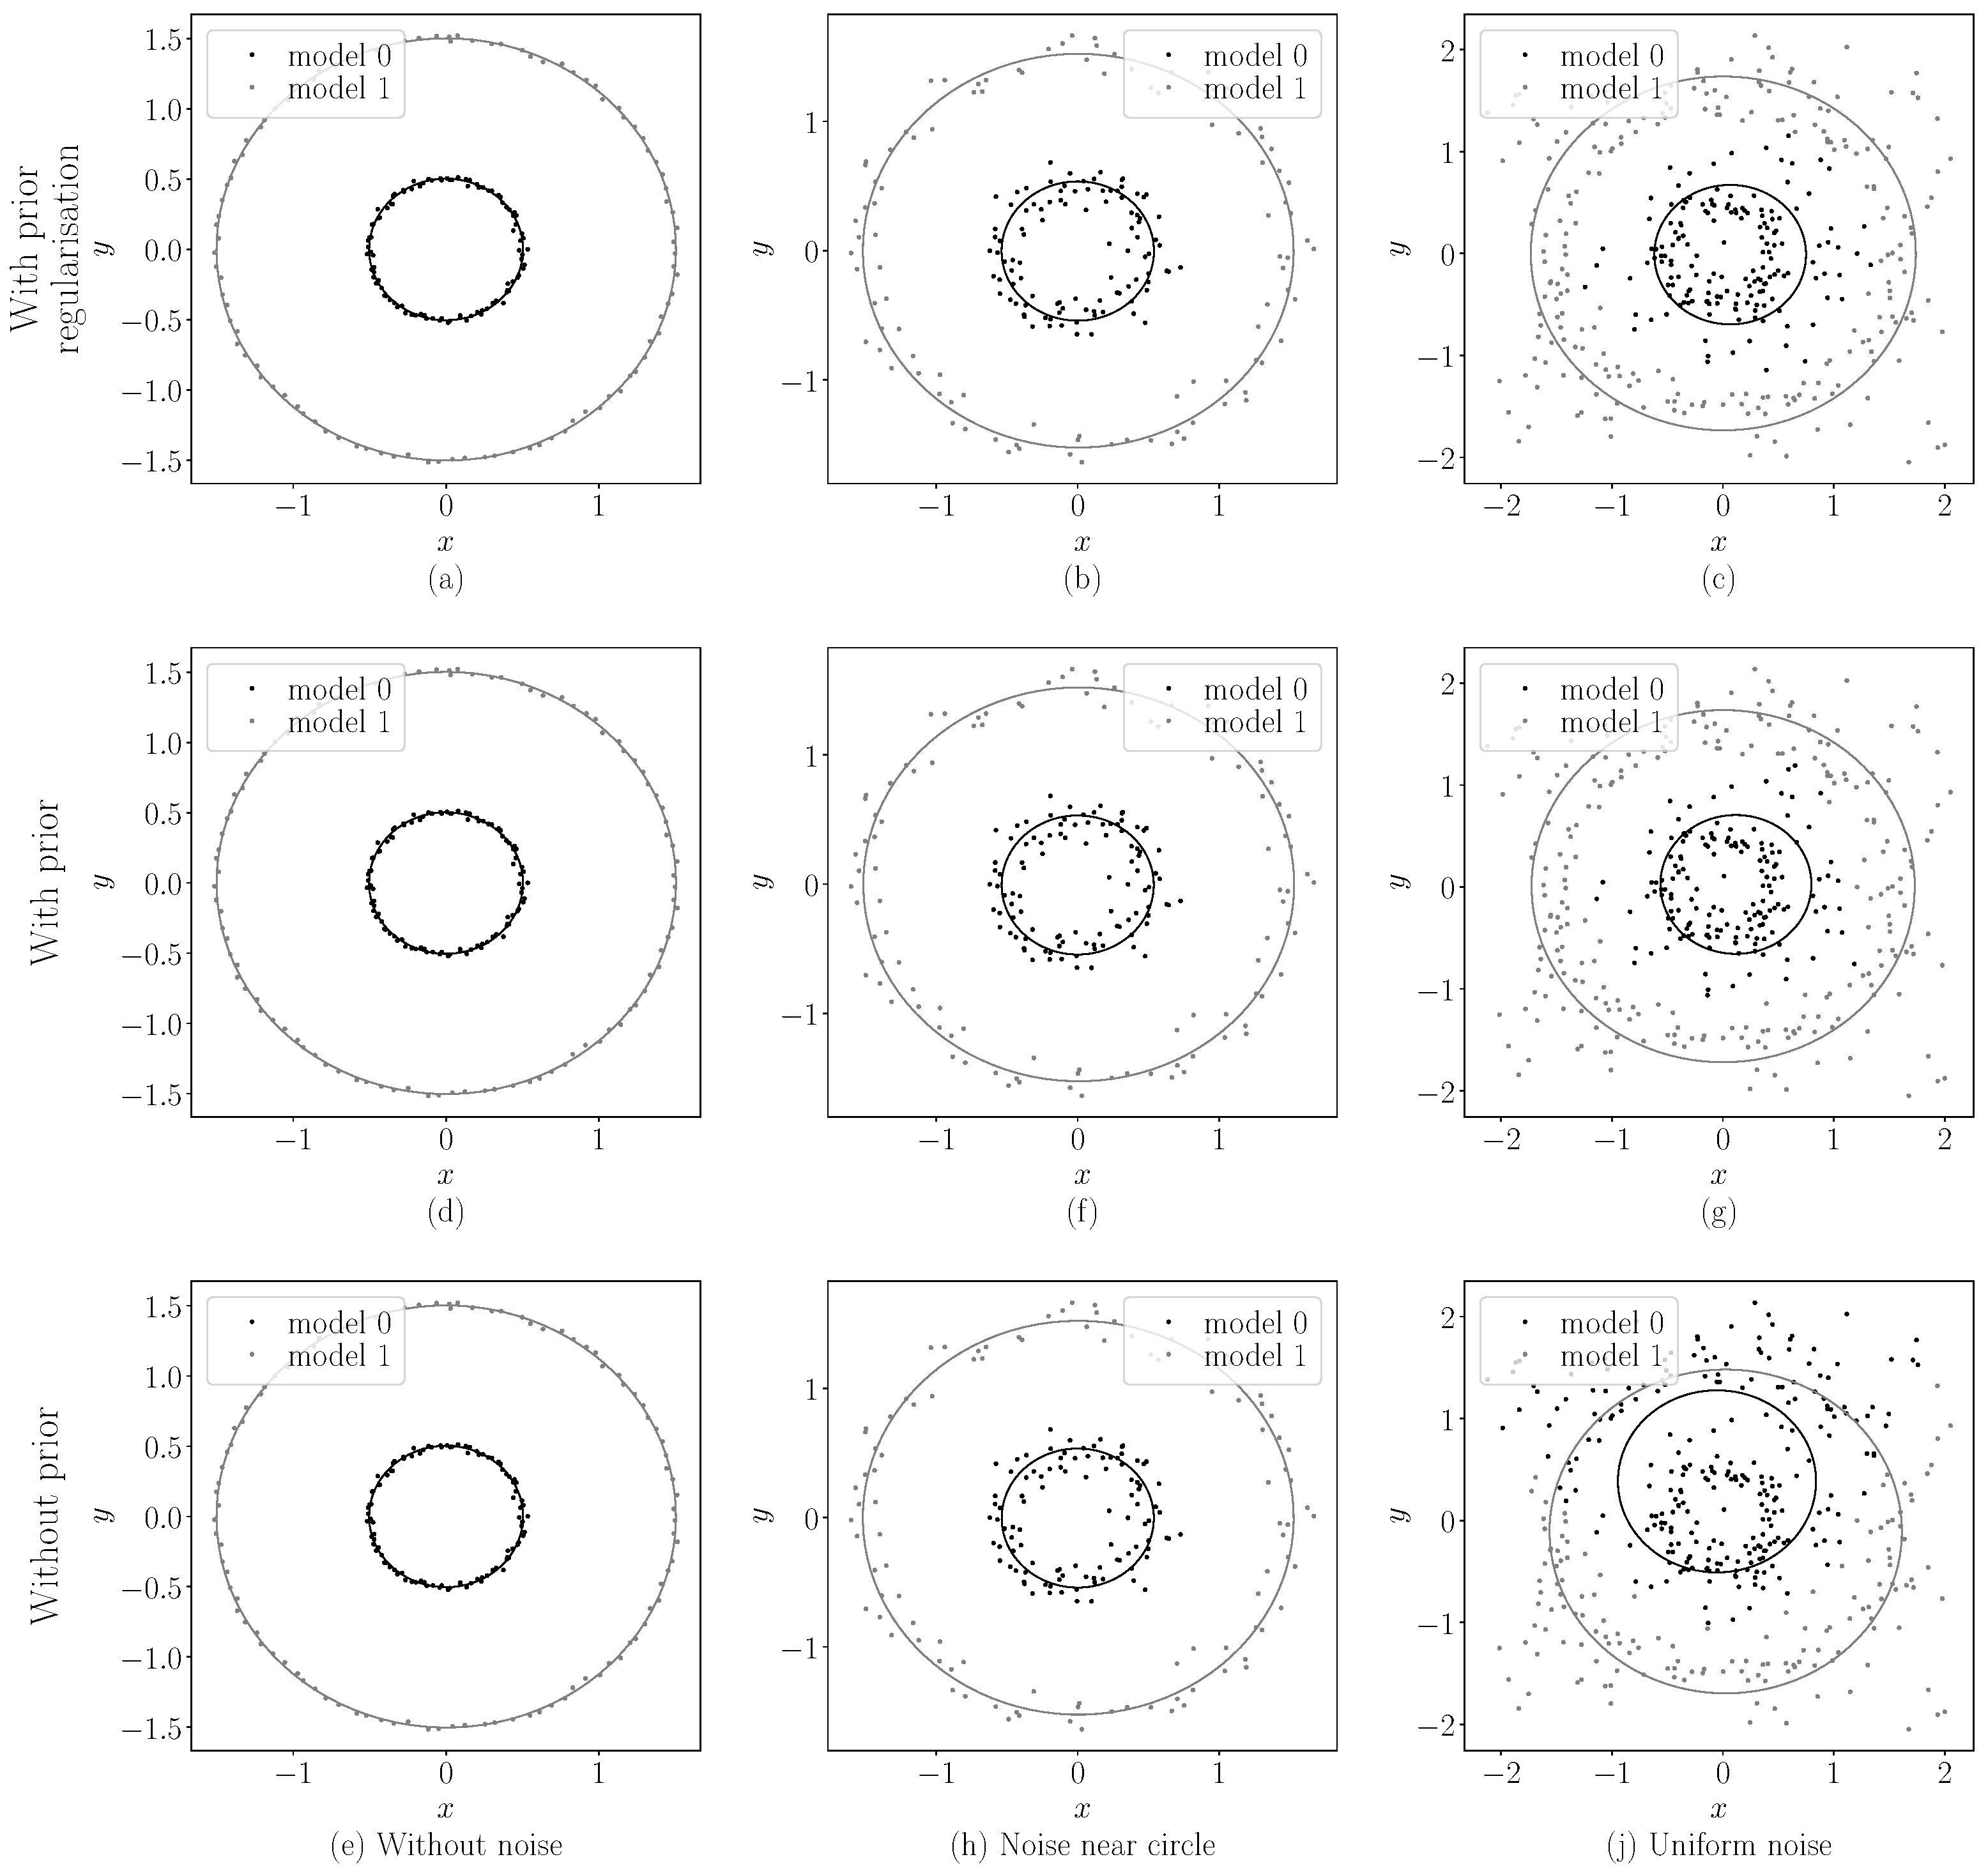
\includegraphics[width=1\textwidth]{results/priorexpert/experiment_synthetic}
\caption{Мультимодель в зависимости от разных априорных предположений и в зависимости от разного уровня шума: (a)--(с) модель с регуляризаций априорных распределений; (d)--(g) модель с заданными априорными распределениями на параметрах локальных моделей; (e)--(j) модель без заданных априорных предположений}
\label{experiment:1}
\end{figure}
В вычислительном эксперименте сравнивается качество следующих мультимоделей $\textbf{f}_1, \textbf{f}_2, \textbf{f}_3$ на синтетических данных.
Синтетические данные являются двумя концентрическими окружностями с разным уровнем шума.
Выборка Synthetic 1 является изображением без шума, выборка Synthetic 2 изображение с зачумлённым радиусом окружности, а выборка Synthetic 3 --- изображение с равномерным шумом.
На рис. \ref{experiment:1} показаны результаты для мельтимоделей $\textbf{f}_1, \textbf{f}_2, \textbf{f}_3$.
Все модели оптимизировались при помощи 50 итераций EM-алгоритма.
Мультимодели $\textbf{f}_2, \textbf{f}_3$ аппроксимируют окружности лучше чем мультимодель $\textbf{f}_1$. В табл. \ref{tb:ce:1} показано качество аппрроксимации \eqref{eq:ce:ex:0:1} для всех мультимоделей.

\begin{table}[h!t]
\begin{center}
\caption{Качество аппроксимации \eqref{eq:ce:ex:0:1} для всех мультимоделей}
\label{tb:ce:1}
\begin{tabular}{|c|c|c|c|}
\hline
	Выборка & $\mathcal{S}_{\textbf{f}_1}$ & $\mathcal{S}_{\textbf{f}_2} $& $\mathcal{S}_{\textbf{f}_3} $\\
	\hline
	\multicolumn{1}{|l|}{Synthetic 1}
	& $10^{-5}$& $10^{-5}$& $10^{-5}$\\
	\hline
	\multicolumn{1}{|l|}{Synthetic 2}
	& $0.6$& $10^{-3}$& $10^{-3}$\\
	\hline
	\multicolumn{1}{|l|}{Synthetic 3}
	& $0.6$& $10^{-3}$& $10^{-3}$\\
\hline
\end{tabular}
\end{center}
\end{table}

\paragraph{Анализ сходимости на синтетической выборке.}
\begin{figure}[h!t]\center
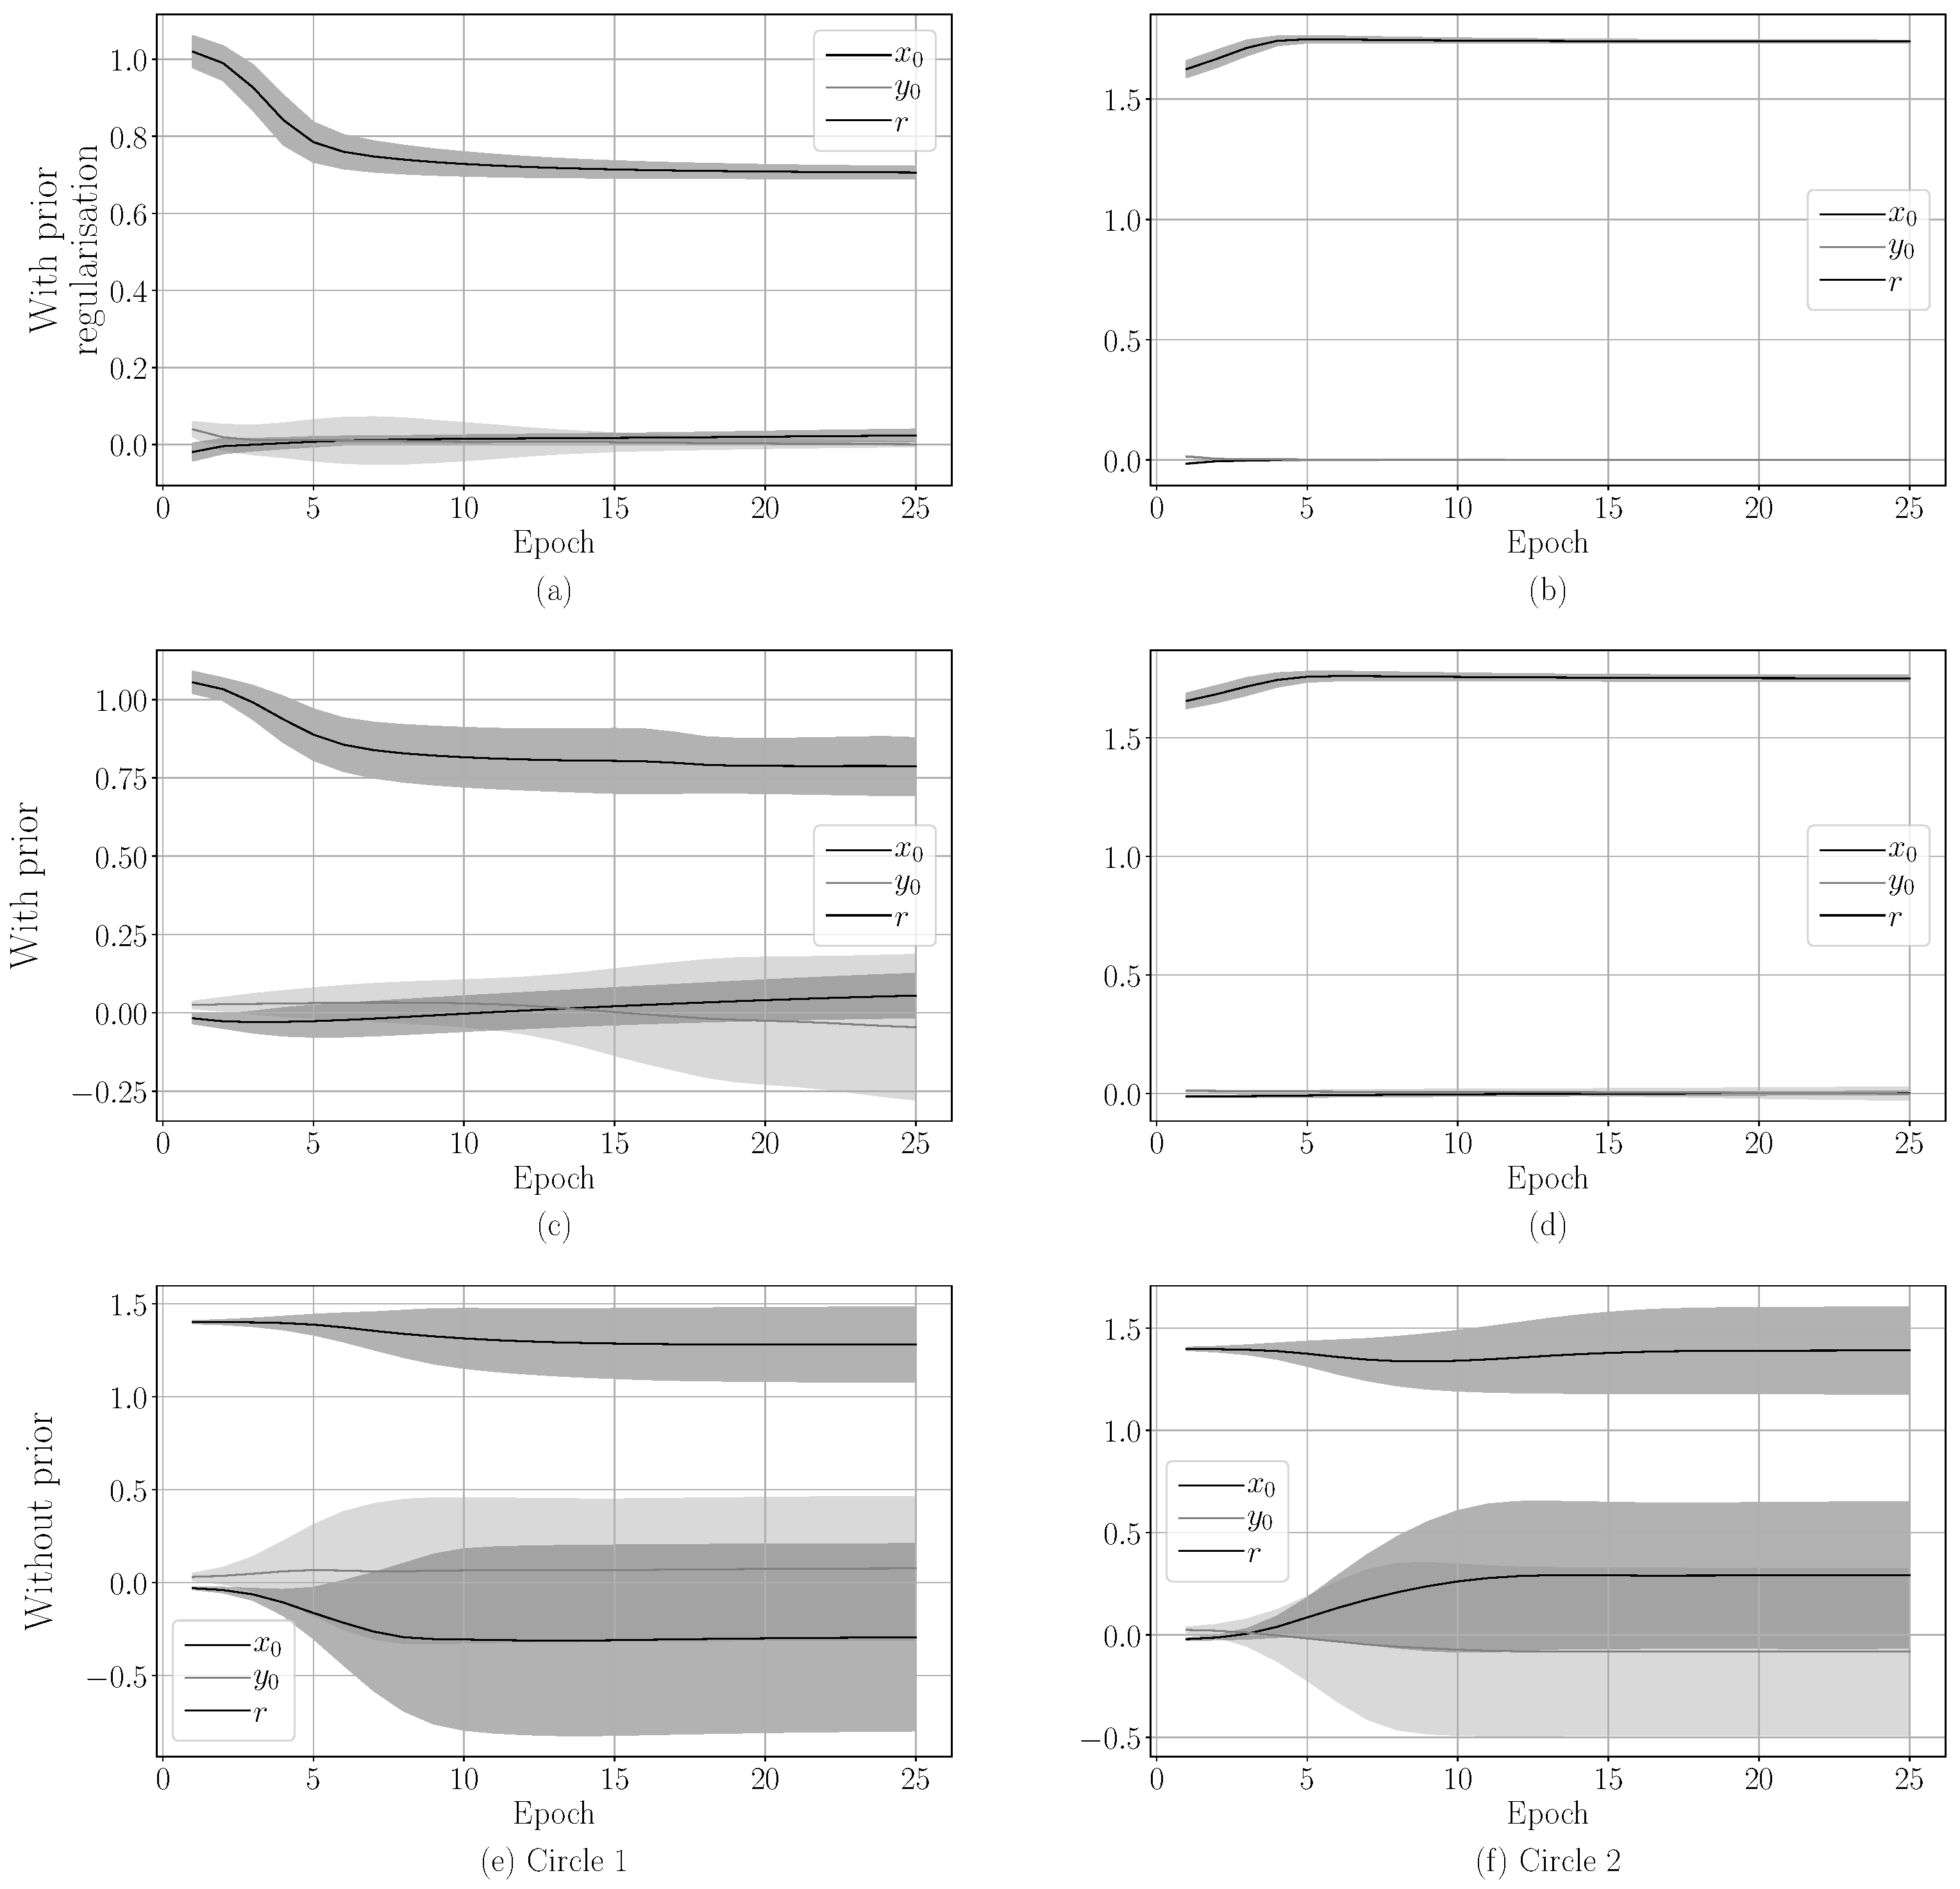
\includegraphics[width=1\textwidth]{results/priorexpert/experiment_synthetic_param_progress}
\caption{График зависимости центра и радиуса окружностей от номера итерации: (a)--(b) модель с регуляризацией априорных распределений; (c)--(d) модель с заданными априорными распределениями на параметры моделей; (e)--(f) модель без задания априорных распределений}
\label{experiment:st:2:1}
\end{figure}

\begin{figure}[h!t]\center
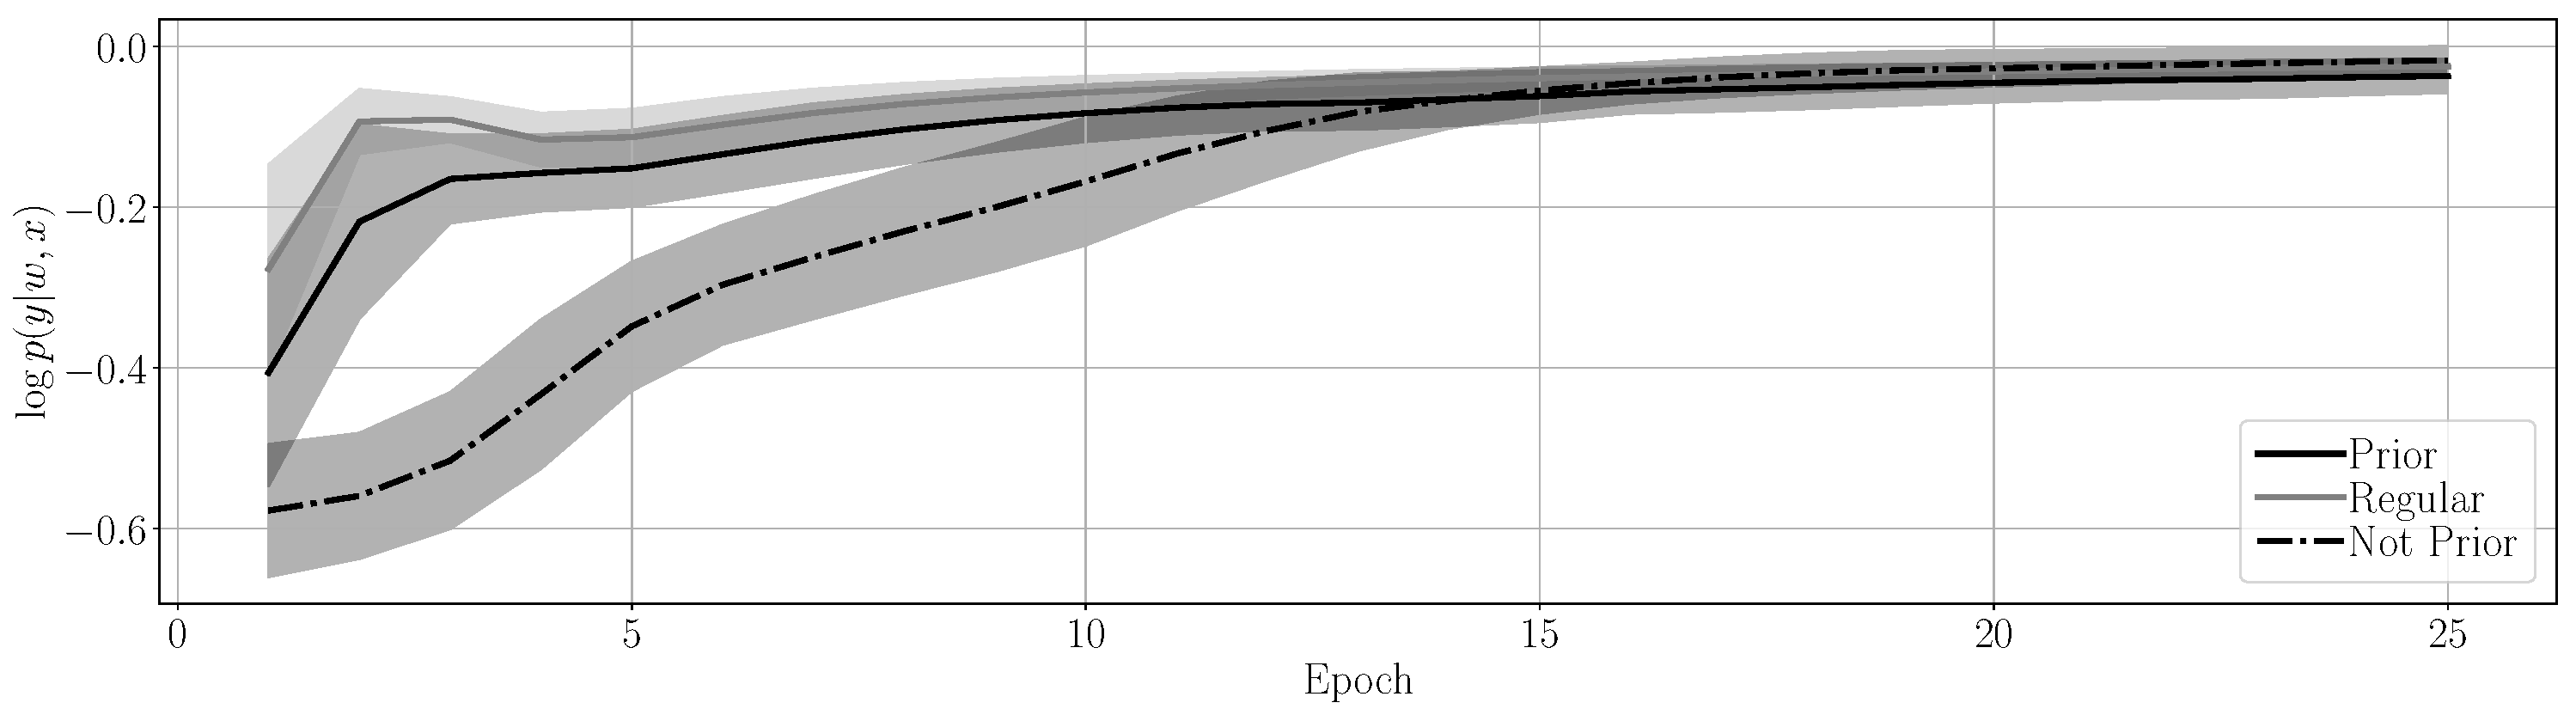
\includegraphics[width=1\textwidth]{results/priorexpert/experiment_synt_likelihood_progress}
\caption{График зависимости логарифма правдоподобия \eqref{eq:st:new:1} от номера итерации.}
\label{experiment:st:2:2}
\end{figure}

\begin{figure}[h!t]\center
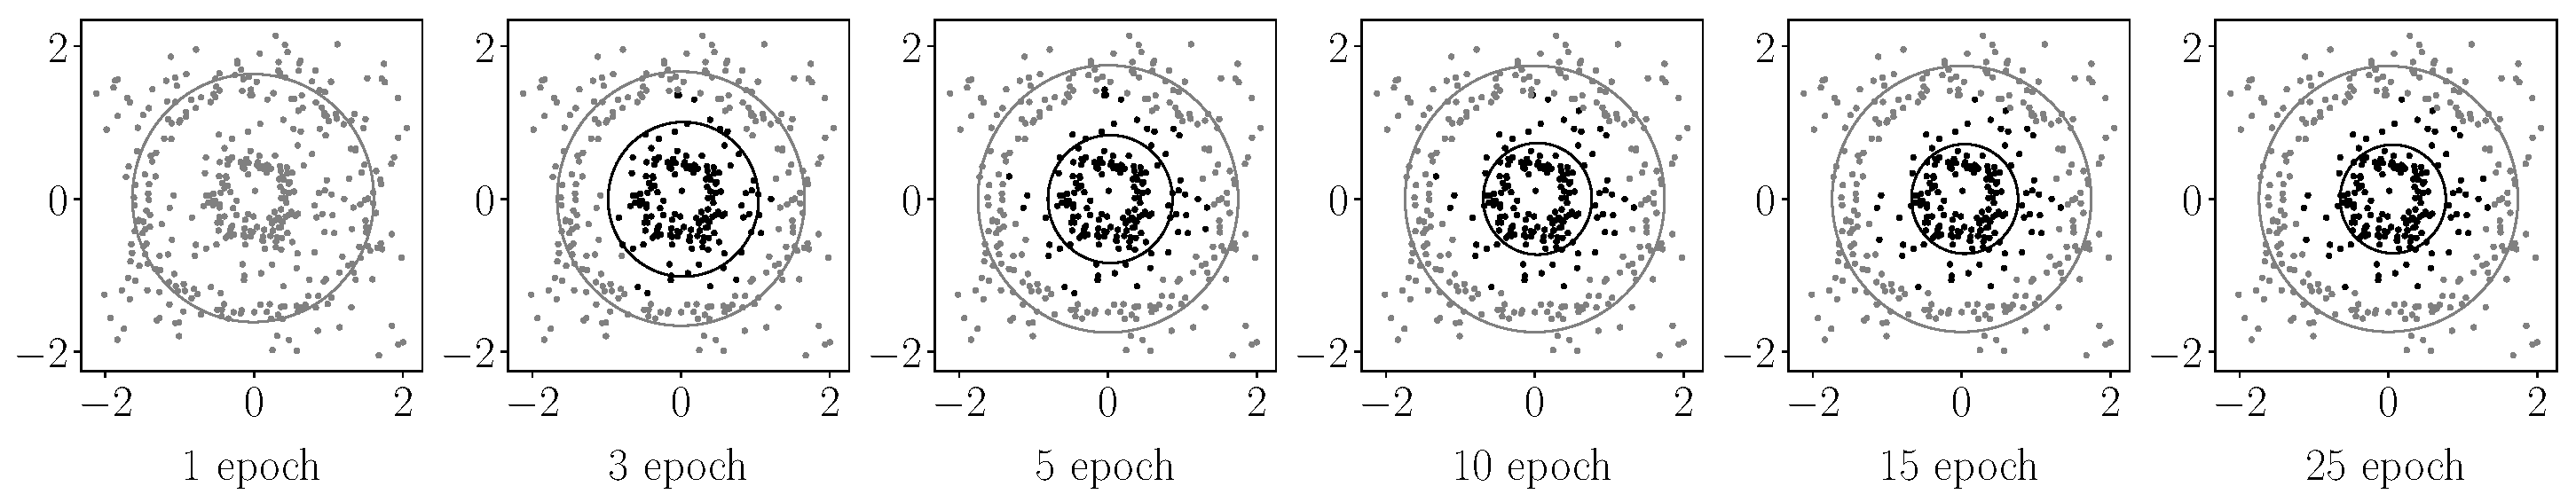
\includegraphics[width=1\textwidth]{results/priorexpert/experiment_synt_regular_progress}
\caption{Визуализации процесса сходимости мультимодели с использованием априорной регуляриции.}
\label{experiment:st:2:3}
\end{figure}

\begin{figure}[h!t]\center
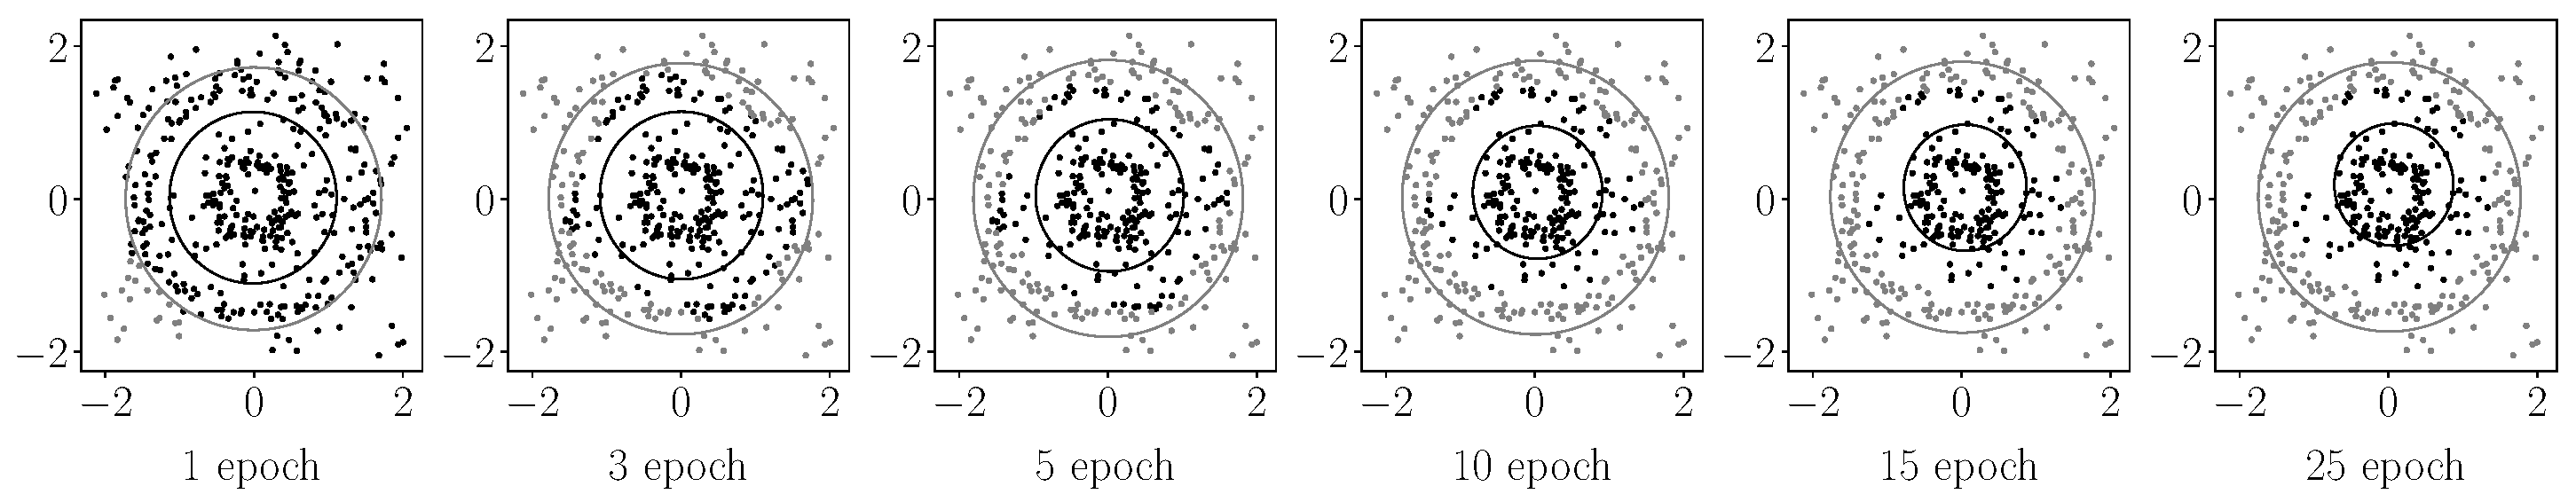
\includegraphics[width=1\textwidth]{results/priorexpert/experiment_synt_prior_progress}
\caption{Визуализации процесса сходимости мультимодели с использованием априорного распределением.}
\label{experiment:st:2:4}
\end{figure}

\begin{figure}[h!t]\center
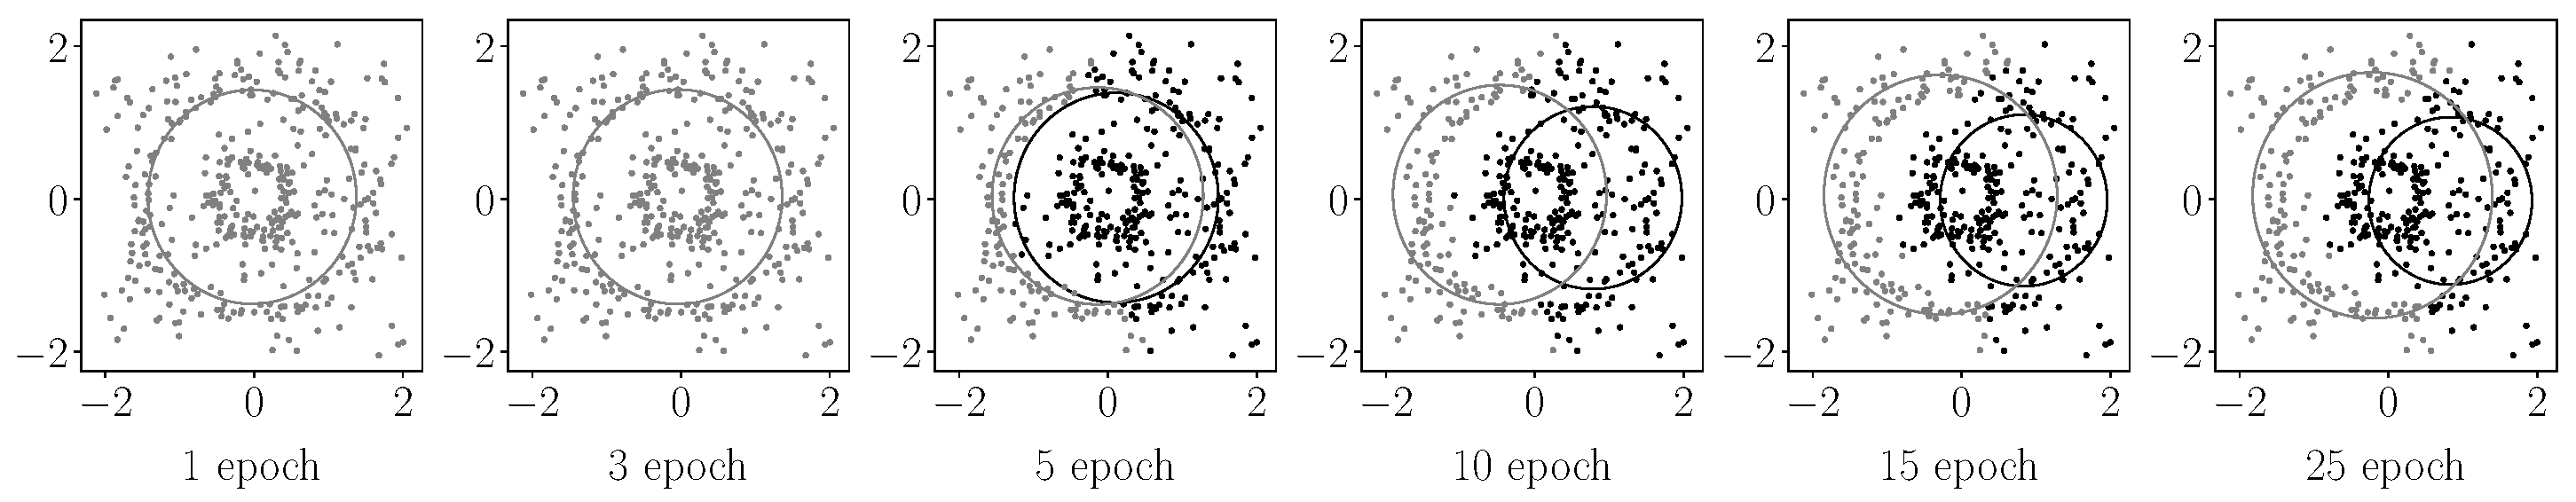
\includegraphics[width=1\textwidth]{results/priorexpert/experiment_synt_not_prior_progress}
\caption{Визуализации процесса сходимости мультимодели без использования априорного распределения.}
\label{experiment:st:2:5}
\end{figure}
Данная часть эксперимента анализирует качество сходимости ЕМ-алгоритма для разных мультимоделей $\textbf{f}_1, \textbf{f}_2, \textbf{f}_3$.
Анализ всех мультимоделей проводиться на выборке Synthetic 3.

На рис. \ref{experiment:st:2:1} показана зависимость предсказано центра и радуса в зависимости от номера итерации ЕМ-алгоритма.
Мультимодель $\textbf{f}_2,$ которая использует априорное распределение аппроксимирует окружность лучше мультимодели $\textbf{f}_1,$ которая не использует никакого априорного распределения.
Мультимодель $\textbf{f}_3,$ которая использует регуляризатор априорных распределений является более стабильной, чем мультимодель $\textbf{f}_2$.

На рис. \ref{experiment:st:2:2} показана зависимость логарифма правдоподобия \eqref{eq:st:new:1} от номера итерации EM-алгоритма.
Логарифм правдоподобия мультимодели $\textbf{f}_2, \textbf{f}_3$ растет быстрее чем логарифм правдоподобия мультимодели $\textbf{f}_1$.  После $20$-й итерации все мультимодели имеют одинаковое правдоподобие.

На рис. \ref{experiment:st:2:3}-\ref{experiment:st:2:5} показан процесс сходимости для разных мультимоделей $\textbf{f}_1, \textbf{f}_2, \textbf{f}_3$.
На рис. \ref{experiment:st:2:5} показана мультимодель $\textbf{f}_1$, которая аппроксимирует окружности не верно.
На рис. \ref{experiment:st:2:3}-\ref{experiment:st:2:4} показаны мультимодели $\textbf{f}_2, \textbf{f}_3$, которые аппроксимируют окружности верно.

Вычислительный эксперимент показывает, что мультимодели $\textbf{f}_2, \textbf{f}_3,$ которые используют априорные распределения на параметры экспертов аппроксимируют окружности лучше чем мультимодель $\textbf{f}_1,$ которая работает без априорных распределений.


\paragraph{Анализ мультимоделей в зависимости от уровня шума.} 
\begin{figure}[h!t]\center
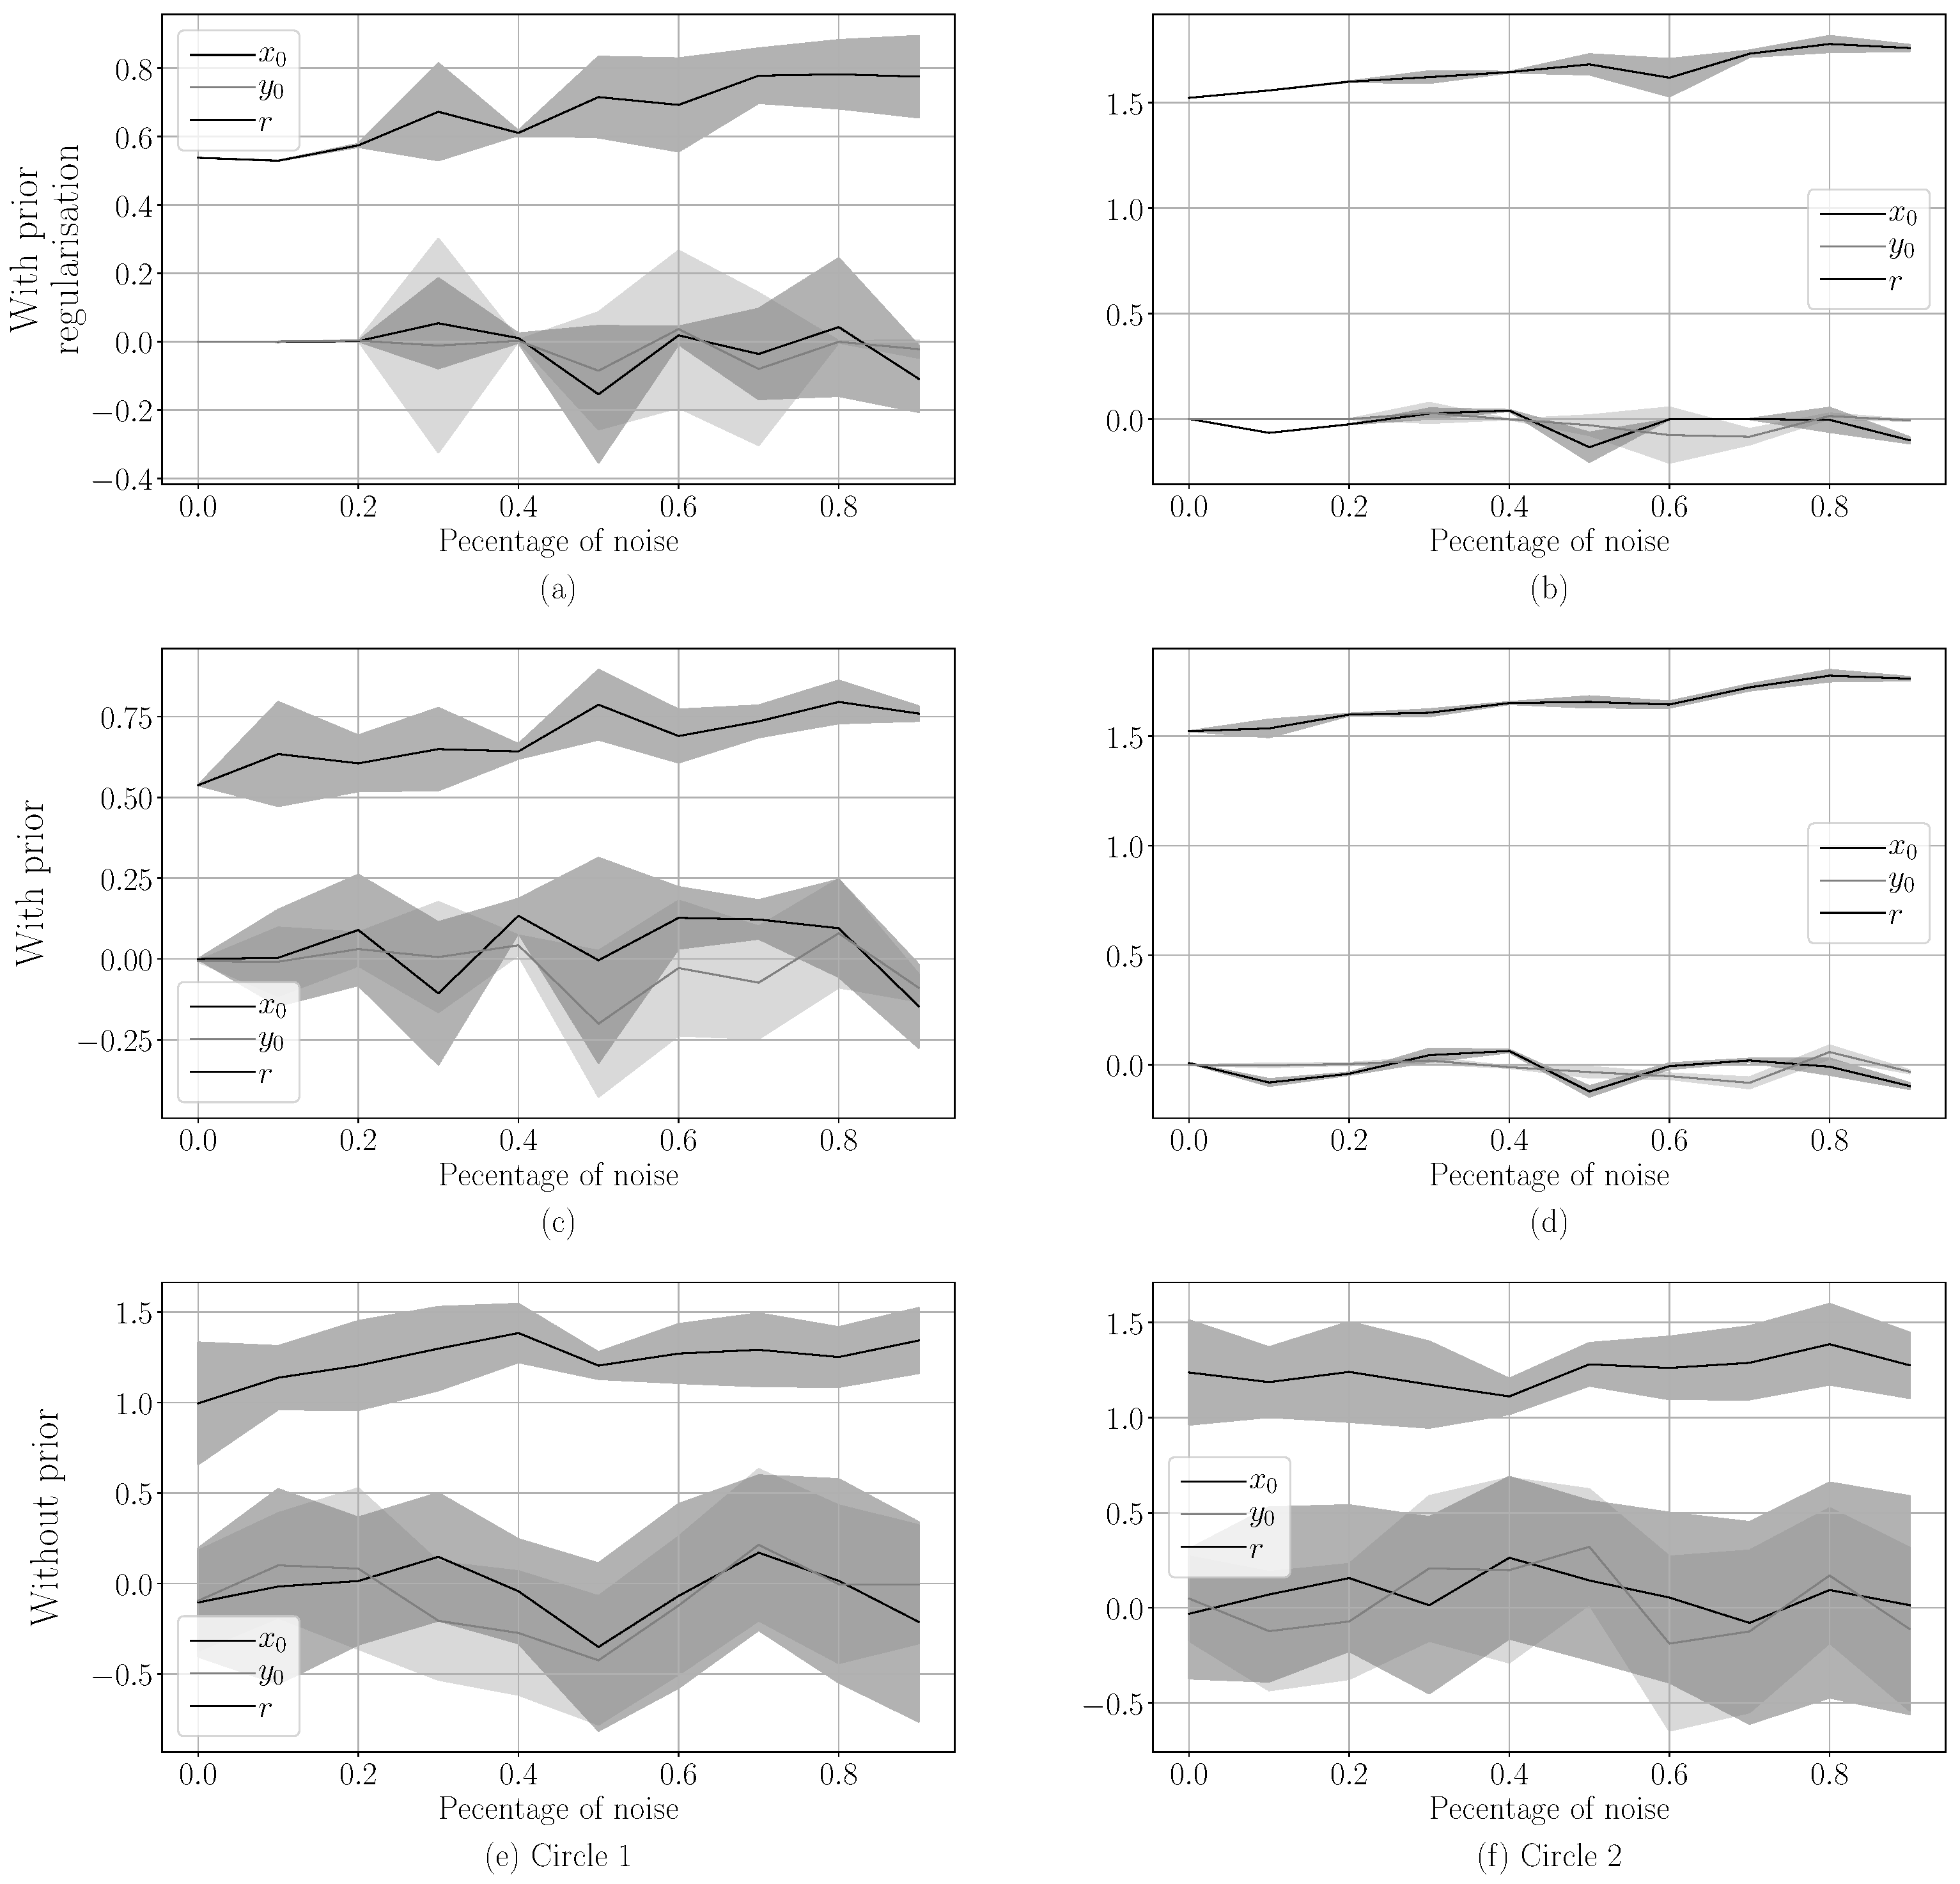
\includegraphics[width=1\textwidth]{results/priorexpert/experiment_synthetic_param_progress_noise}
\caption{рафик зависимости центра и радиуса окружностей от номера итерации: (a)--(b) модель с регуляризацией априорных распределений; (c)--(d) модель с заданными априорными распределениями на параметры моделей; (e)--(f) модель без задания априорных распределений}
\label{experiment:st:3:1}
\end{figure}

\begin{figure}[h!t]\center
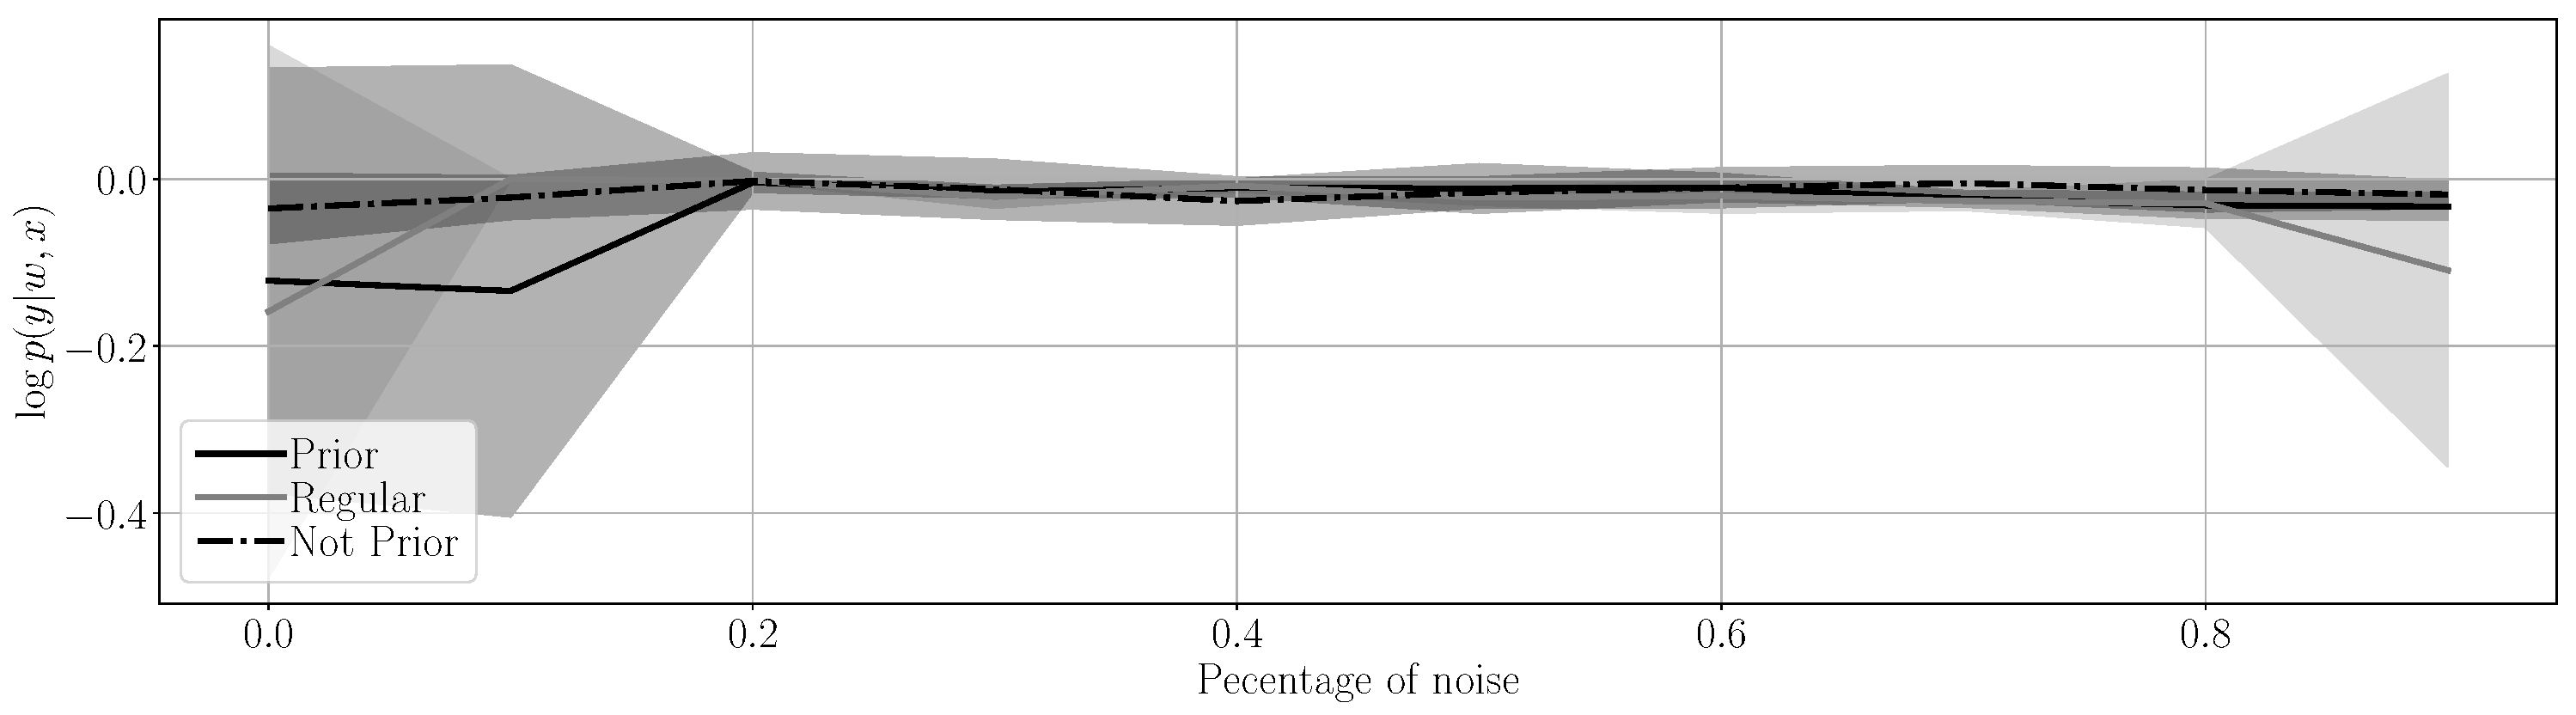
\includegraphics[width=1\textwidth]{results/priorexpert/experiment_synt_likelihood_progress_noise}
\caption{График зависимости логарифма правдоподобия \eqref{eq:st:new:1} от уровня шума.}
\label{experiment:st:3:2}
\end{figure}

Данная часть эксперимента анализирует зависимость разных мультимоделей $\textbf{f}_1, \textbf{f}_2, \textbf{f}_3$ от уровня шума. 
Анализ всех мультимоделей проводиться на выборке Synthetic 1, с добавлением разного уровня шума.
Минимальный уровень шума равен $0$, когда числа шумовых точек равно $0$. Максимальный уровень шума равен $1$, когда число шумовых точек равно числу точек на изображении.
На рис. \ref{experiment:st:3:1} показан график зависимости центра окружности и ее радиус в зависимости от уровня шума. Из графика видно, что радиус окружности увеличивается при увеличении уровня шума. 
Мультимодели $\textbf{f}_2, \textbf{f}_3$ аппроксимируют центр окружности верно, но мультимодель $\textbf{f}_3$ более устойчива к шуму .
На рис. \ref{experiment:st:3:2} показана зависимость логарифма правдоподобия \eqref{eq:st:new:1} от уровня шума. 
Из графика видно, что логарифм правдоподобия \eqref{eq:st:new:1} эквивалентный для всех мультимоделей, но на рис. \ref{experiment:st:3:1} видно, что качество аппроксимации \eqref{eq:ce:ex:0:1} зависит от мультимодели.
Данная часть вычислительного эксперимента показывает, что мультимодель $\textbf{f}_3$ с регуляризацией априорного распределения является более устойчива к шуму, чем остальные.

\paragraph{Реальные данные.}
\begin{figure}[h!t]\center
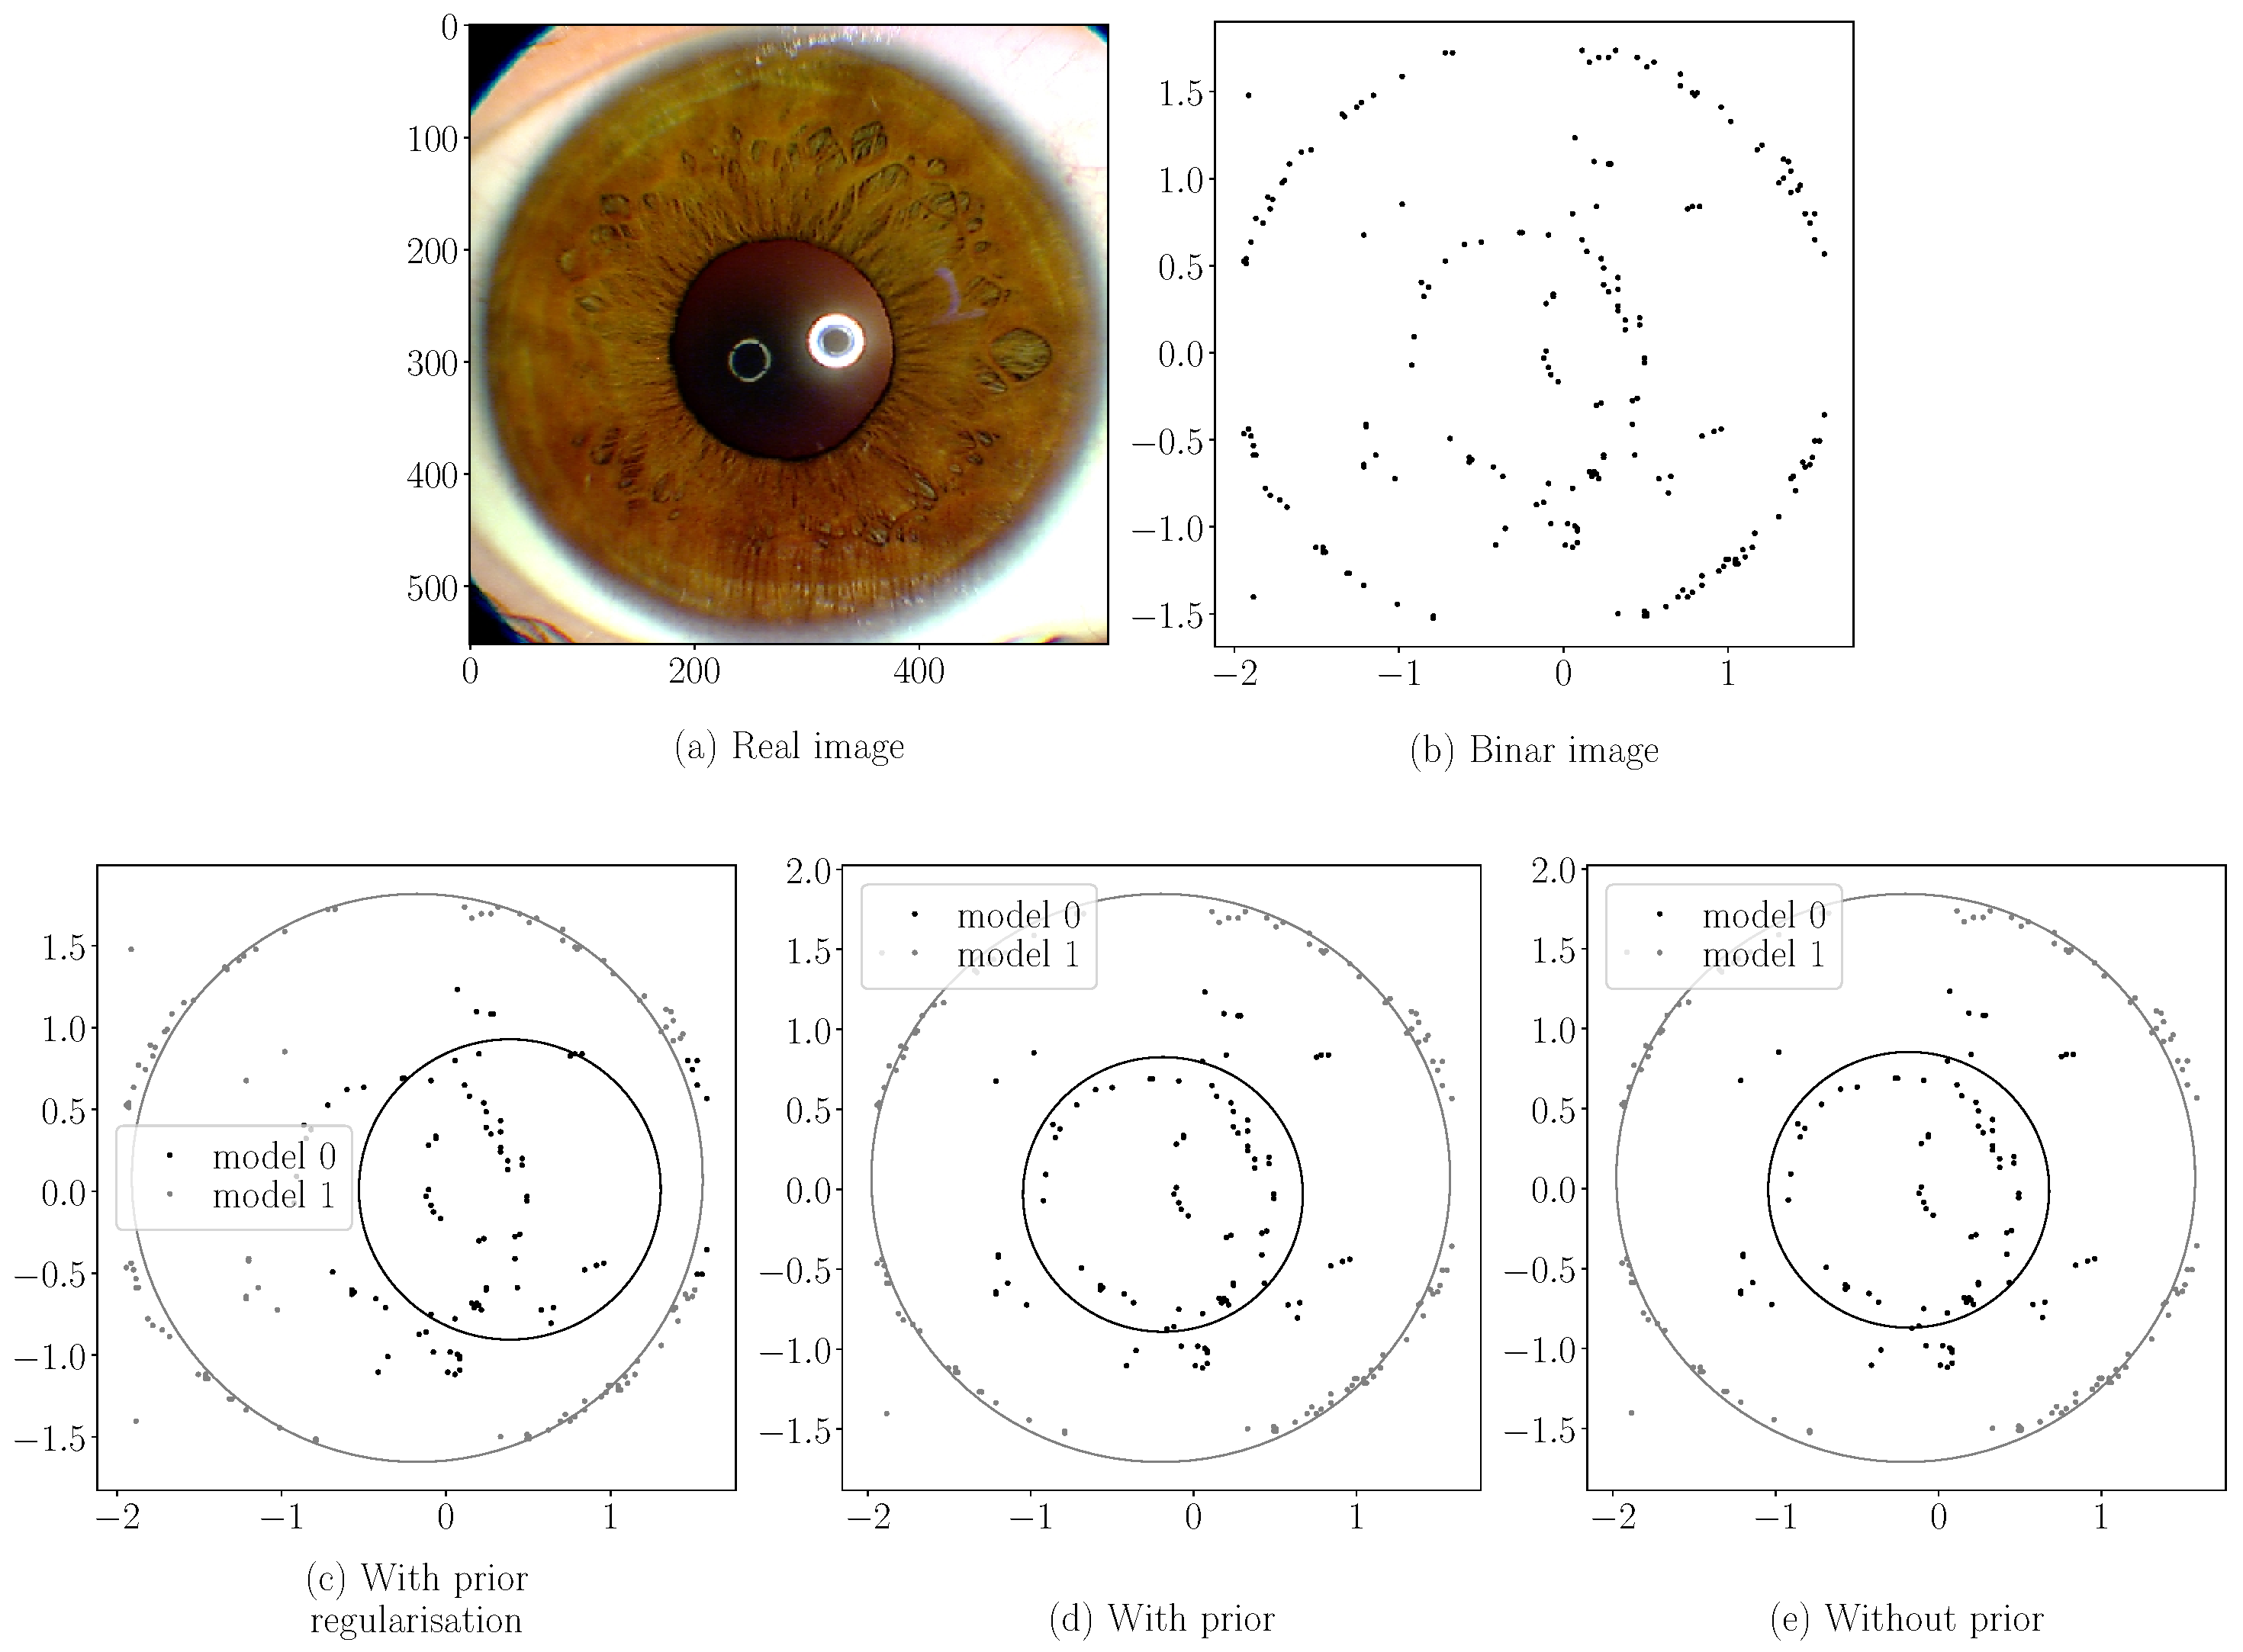
\includegraphics[width=0.9\textwidth]{results/priorexpert/experiment_real_compare}
\caption{Мультимодель в зависимости от разных априорных предположений на реальном изображении: (a) исходное изображение; (b) бинаризованое изображение; (c) мультимодель без априорных предположений; (d) мультимодель с априорными распределениями на параметрах локальных моделей; (e) мультимодель с регуляризаций на априорных распределениях параметров локальных моделей.}
\label{experiment:2}
\end{figure}

Данная часть эксперимента анализирует разные мультимодели $\textbf{f}_1, \textbf{f}_2, \textbf{f}_3$ на реальной выборке.
На рис. \ref{experiment:2} показан результат работы разных мультимоделей.
Мультимодель $\textbf{f}_1$  не верно аппроксимирует меньшую окружность.
Мультимодели $\textbf{f}_2, \textbf{f}_3$ аппроксимируют обе окружности верно.

\begin{figure}[h!t]\center
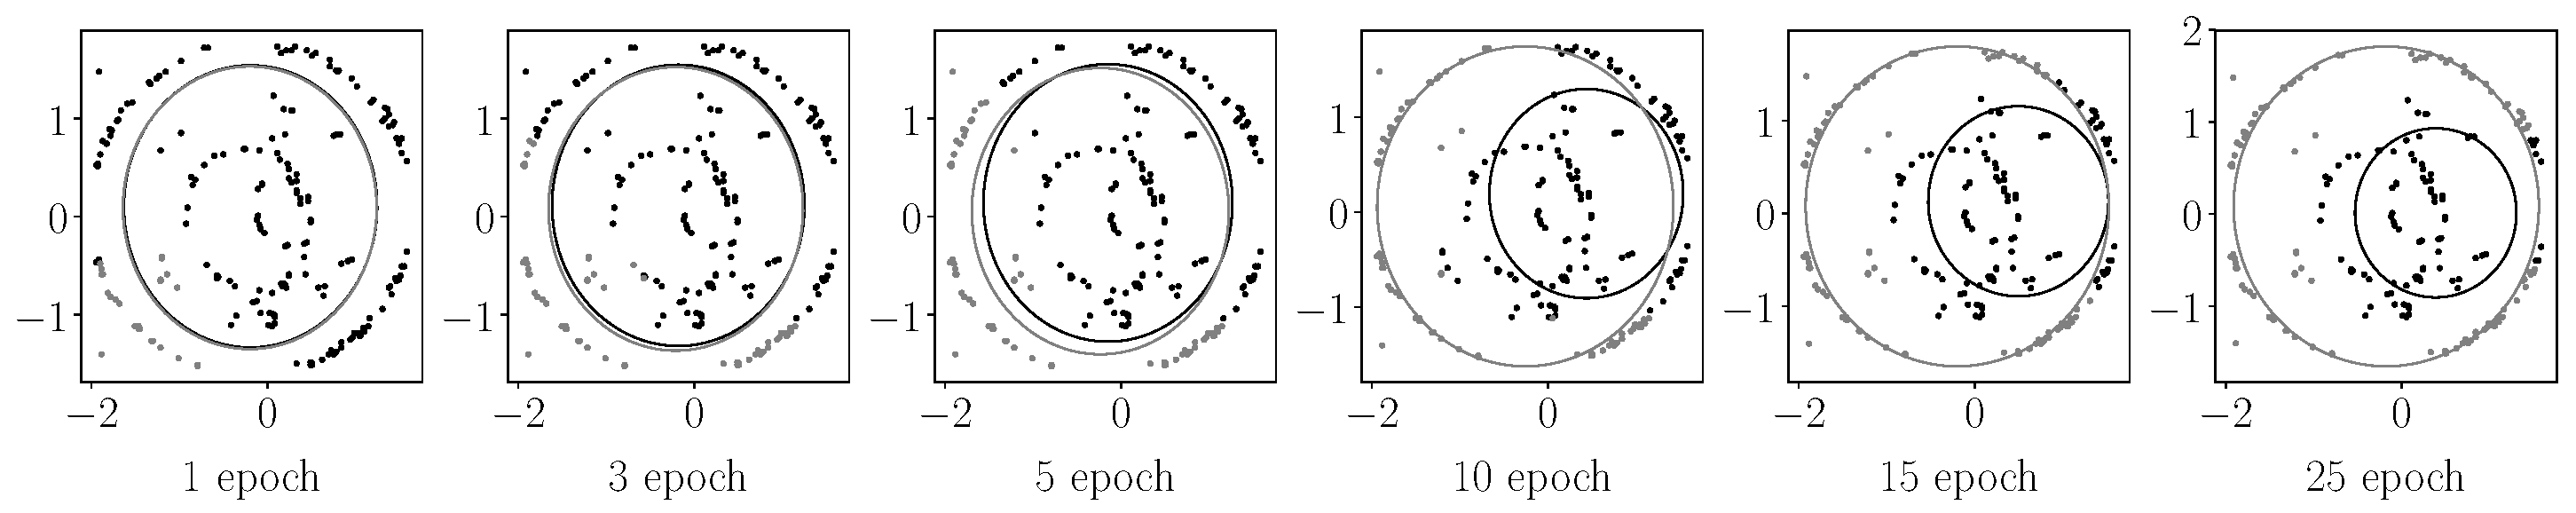
\includegraphics[width=1\textwidth]{results/priorexpert/experiment_real_not_prior}
\caption{Визуализации процесса сходимости мультимодели без использования априорного распределения.}
\label{experiment:3}
\end{figure}

\begin{figure}[h!t]\center
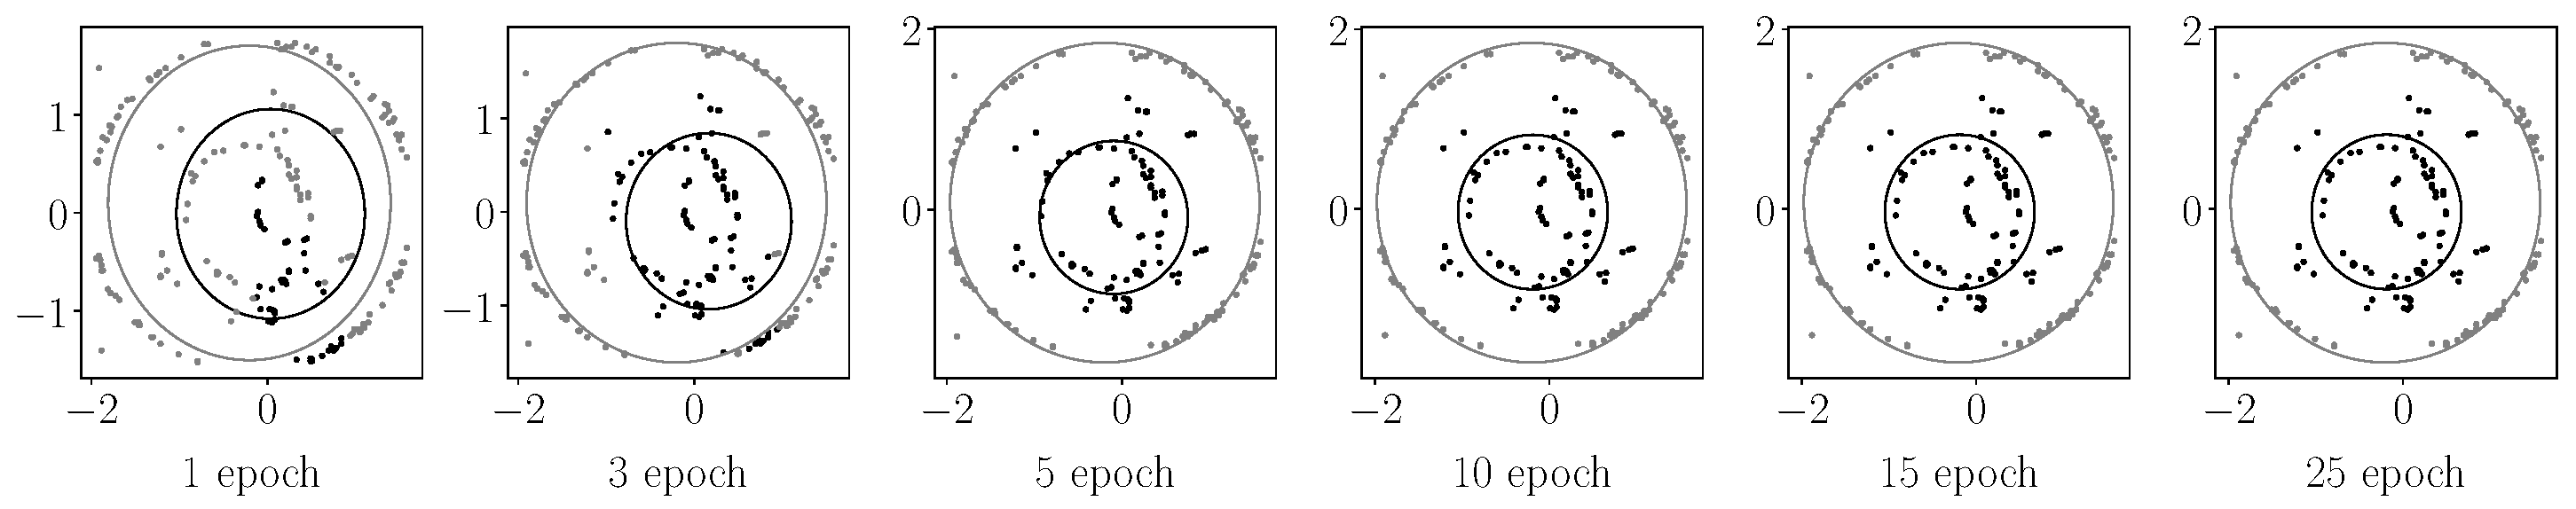
\includegraphics[width=1\textwidth]{results/priorexpert/experiment_real_prior}
\caption{Визуализации процесса сходимости мультимодели с использованием априорного распределением.}
\label{experiment:4}
\end{figure}

\begin{figure}[h!t]\center
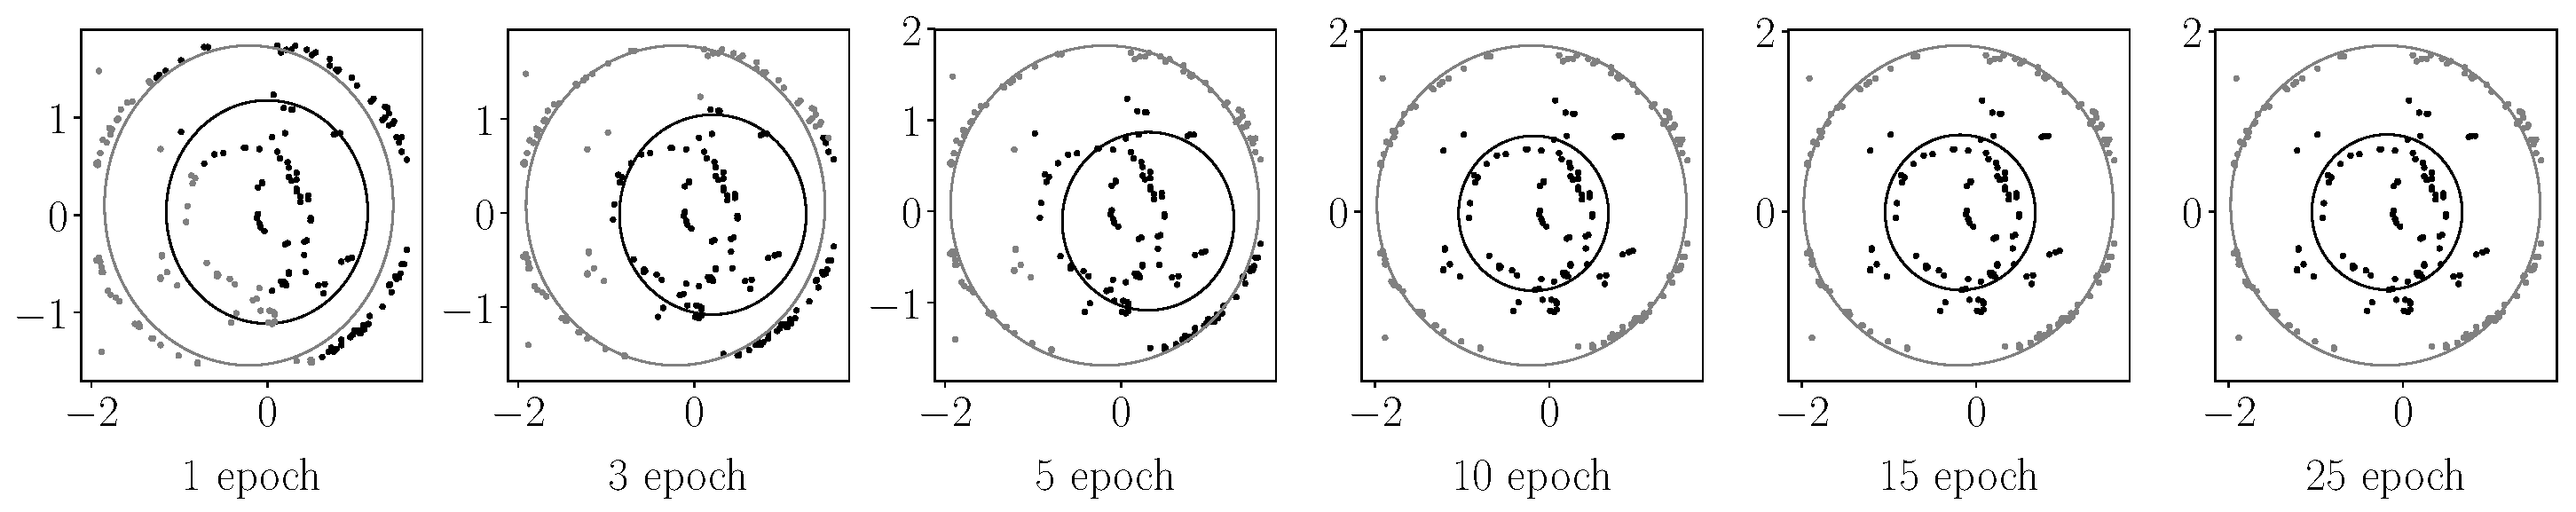
\includegraphics[width=1\textwidth]{results/priorexpert/experiment_real_regular}
\caption{Визуализации процесса сходимости мультимодели с использованием априорной регуляриции.}
\label{experiment:5}
\end{figure}

На рис. \ref{experiment:3}-\ref{experiment:5} показан процесс аппроксимации для разных мультимоделей $\textbf{f}_1, \textbf{f}_2, \textbf{f}_3$.

Данная часть эксперимента показывает, что мультимодели $\textbf{f}_2, \textbf{f}_3$ аппроксимируют окружности на реальных изображениях лучше, чем мультимодель $\textbf{f}_1$.